% Main file: main.tex
% Compile this file to build the full document

\documentclass[a4paper,12pt,twoside]{report} % Use book class for structured documents
\usepackage[square]{natbib}          % Bibliography support
\renewcommand{\citepunct}{; }
\usepackage[utf8]{inputenc}          % Support for UTF-8 characters
\usepackage{amsmath, amssymb}        % Mathematical symbols and equations
\usepackage{amsthm}                  % For theorem-like environments
\usepackage{graphicx, animate}       % For including images and animations
\usepackage[font=small, labelfont=bf]{caption}
\usepackage{subcaption}              % Provides subfigure support
% \usepackage{ragged2e}                % Provides \RaggedRight
\usepackage{etoolbox}
\usepackage{hyperref}                % For hyperlinks



\usepackage[english]{babel}
\usepackage{geometry}                % Page layout customization
\usepackage{titlesec}                % For customizing section titles
\usepackage{fancyhdr}
\usepackage[table]{xcolor}
\usepackage{tabularx}
% \usepackage{cite}
\usepackage{xcolor}
\newcommand{\highlight}[1]{\colorbox{yellow}{#1}} % Custom highlight command
\usepackage{soul}                    % For colour management
\usepackage[nottoc]{tocbibind}       % Includes "References" in ToC
\usepackage{algorithm}               % For writing algorithms
\usepackage{algorithmic}             % For algorithmic environments
\renewcommand{\thealgorithm}{\thesection.\arabic{algorithm}}  % Modify algorithm number to include section number

% Defining argmin and argmax operator
% -----------------------------------
\DeclareMathOperator*{\argmax}{arg\,max}
\DeclareMathOperator*{\argmin}{arg\,min}

% Define a new theorem style for definitions
% ------------------------------------------
\newtheoremstyle{definition}
  {10pt} % Space above
  {10pt} % Space below
  {\normalfont} % Body font
  {} % Indent amount
  {\bfseries} % Theorem head font
  {.} % Punctuation after theorem head
  {.5em} % Space after theorem head
  {} % Theorem head spec (can be left empty, meaning 'normal')

\theoremstyle{definition}
\newtheorem{definition}{Definition}[section]

% Define a new theorem style for propositions
% ------------------------------------------
\newtheoremstyle{proposition}
  {10pt} % Space above
  {10pt} % Space below
  {\normalfont} % Body font
  {} % Indent amount
  {\bfseries} % Theorem head font
  {.} % Punctuation after theorem head
  {.5em} % Space after theorem head
  {} % Theorem head spec (can be left empty, meaning 'normal')

\theoremstyle{proposition}
\newtheorem{proposition}{Proposition}[section]

% Define a new theorem style for examples
% ------------------------------------------
\newtheoremstyle{example}
  {10pt} % Space above
  {10pt} % Space below
  {\normalfont} % Body font
  {} % Indent amount
  {\bfseries} % Theorem head font
  {.} % Punctuation after theorem head
  {.5em} % Space after theorem head
  {} % Theorem head spec (can be left empty, meaning 'normal')

\theoremstyle{example}
\newtheorem{example}{Example}[section]


% Page layout settings
\geometry{margin=1in}

% Customizing Chapter Heading Style
\titleformat{\chapter}[block] % 'block' means the title will be on its own line
  {\normalfont\huge\bfseries} % Font settings for the chapter title
  {\thechapter}               % Numbering format (e.g., "1")
  {1em}                       % Space between the number and title
  {}                          % No prefix for the chapter title



\begin{document}

\pagestyle{fancy}
\fancyhead{}                                 % clear all header fields
\fancyfoot{}                                 % clear all footer fields

\fancyhead[LE, RO]{\small\nouppercase{\rightmark}}  % Section/Chapter title on left (even pages)

\fancyfoot[C]{\small\thepage}  % Page number centered in the footer

\renewcommand{\headrulewidth}{0pt}

% Title Page
\title{\textbf{Covariate Shift Regularization with Kernels}}
\author{Suvinava Basak}
\date{\today}
\maketitle

% Blank Page before Summary
\cleardoublepage
% \thispagestyle{empty} % Removes page number

% Customizing Summary Heading Size
\titleformat{\section}[block]
{\normalfont\Huge\bfseries}{}{0pt}{}

% Summary Page
\newpage
\vspace*{5cm} % Push the content to the middle of the page
\section*{Abstract}
% \addcontentsline{toc}{section}{Summary} % Add to Table of Contents
Covariate shift, a fundamental challenge in supervised learning, occurs when the distribution of input features differs between training and test datasets while the conditional distribution of the target given the input remains unchanged. This work explores covariate shift through the lens of kernel-based learning, particularly in linear regression settings. We analyze theoretical foundations, propose strategies for mitigating covariate shift using importance weighting with weights estimated by kernel density estimation and self-attention mechanisms.\\

We conduct experiments using synthetic data to assess the effect of mean shift on model performance, comparing ordinary least squares and gradient descent estimators. Our findings highlight the importance of robust learning strategies in the presence of covariate shift and emphasize the role of kernel-based techniques in domain adaptation and distributionally robust optimization.


% Reverting Section Heading Size
\titleformat{\section}[block]
{\normalfont\large\bfseries}{\thesection}{1em}{}

\titleformat{\subsection}[block]{\normalfont\normalsize\bfseries}{\thesubsection}{1em}{}

% Settings for the entire document
\setlength{\parskip}{0em}           % Adds vertical space b/w paragraphs
\setlength{\parindent}{0pt}         % Remove paragraph indent


% Table of Contents
\newpage
\tableofcontents
\newpage



% Include chapters
\chapter{Introduction}\label{chp:1}

\highlight{Lorem Ipsum} % Introduction
\chapter{Covariate Shift}\label{chp:2}

Formally, let $\mathcal{X} \in \mathbb{R}^d$ be the input space from which samples $x$ are drawn and $\mathcal{Y} \in \mathbb{R}$ (or $\mathcal{Y} \in \{0,1\}$ in classification tasks) be the output space. In the standard supervised learning setting, we have access to a training dataset $\{(x_i, y_i)\}_{i=1}^n$ samples from the joint distribution $\mathbb{P}_{\text{train}}(X, Y)$ and we aim to learn a function $f: \mathbb{R}^d \rightarrow \mathbb{R}$ that generalizes well to the new, unseen data from the test distribution $\mathbb{P}_{\text{test}}(X, Y)$. We do that by selecting the function $f: \mathcal{X} \to \mathcal{Y}$ that minimizes the \emph{expected risk}:

$$\mathcal{R}(f) = \mathbb{E}_{\mathbb{P}_{\text{train}}(\mathcal{X},\mathcal{Y})}[\ell(f(X; \theta), Y)]$$

where, $\ell: \mathbb{R} \times \mathbb{R} \to \mathbb{R}$ is a suitable loss function and $\theta$ is the parameter that we aim to learn.\\

Covariate shift occurs when (1) the marginal distribution of the input features (covariates) $X$ differs between the training and testing phases, while (2) the conditional distribution of the output given the input $\mathbb{P}(Y \mid X)$ remains unchanged. This means that while the relationship between the input features and the target variable doesn't change, the way the input features are distributed does. Mathematically, we can break it down as below.\\

Let us define the training and test distributions by $\mathbb{P}_{\text{train}}(X, Y)$ and $\mathbb{P}_{\text{test}}(X, Y)$ respectively. Then under covariate shift, it holds that:

\begin{itemize}
    \item \textbf{Input Distribution Change}: The probability distribution $\mathbb{P}(X)$ of the input variables $X$ changes between training and testing.
    $$\mathbb{P}_{\text{train}} (X) \neq \mathbb{P}_{\text{test}} (X)$$
    \item \textbf{Conditional Distribution Stability}: The conditional distribution $\mathbb{P}(Y \mid X)$ of the target variable $Y$ given the input variables $X$ remains the same.
    $$\mathbb{P}_{\text{train}}(Y \mid X) = \mathbb{P}_{\text{test}}(Y \mid X)$$
\end{itemize}

This mismatch between $\mathbb{P}_{\text{train}} (X)$ and $\mathbb{P}_{\text{test}} (X)$ can degrade the model performance to a great extent, as standard empirical risk minimization (ERM) minimizes the risk under $\mathbb{P}_{\text{train}} (X)$ rather than $\mathbb{P}_{\text{test}} (X)$. In other words, the model was trained on a different distribution of input features. The model may not generalize well if the training data does not adequately represent the test data. Our goal is to adjust for this change while learning the function $f: \mathbb{R}^d \rightarrow \mathbb{R}$ during model training based on the data ${(x_i, y_i)}_{i=1}^{n} \sim \mathbb{P}_{\text{train}}(X, Y)$.

\section{Covariate Shift in Kernel Methods}\label{kernel}

Kernel methods operate by embedding input data $X \in \mathbb{R}^d$ into a high-dimensional feature space $\mathcal{H}$ through a mapping function $\phi: \mathbb{R}^d \to \mathcal{H}$, where $\mathcal{H}$ is a reproducing kernel Hilbert space (RKHS) with inner product $\langle \cdot, \cdot \rangle_{\mathcal{H}}$. Algorithms such as kernel ridge regression (KRR), support vector machines (SVMs), and Gaussian processes (GPs) operate in such RKHS \citep{scholkopf2002learning}. Instead of explicitly computing the mapping $\phi(X)$, kernel methods compute inner products in the feature space using a \textbf{kernel function} $k: \mathbb{R}^d \times \mathbb{R}^d \to \mathbb{R}$:
$$k(X_i, X_j) = \langle \phi(X_i), \phi(X_j) \rangle_{\mathcal{H}}$$

\textbf{Note}: A Reproducing Kernel Hilbert Space (RKHS) is a special type of Hilbert space that is associated with a kernel function and has reproducing property. For any function $f$ in RKHS and any point $x$, we have:

$$f(x) = \langle f, K(x, \cdot) \rangle_{\mathcal{H}}$$

This means that evaluating $f(x)$ is equivalent to taking an inner product with the kernel function.\\

Common kernel functions include:
\begin{itemize}
    \item \textbf{Linear kernel}: $k(X_i, X_j) = X_i^\top X_j$
    \item \textbf{Radial Basis Function (RBF) kernel}: $k(X_i, X_j) = \exp (-\gamma \lVert X_i - X_j\rVert^2)$
    \item \textbf{Polynomial kernel}: $k(X_i, X_j) = (X_i^\top X_j + c)^d$, where $d$ is the degree of polynomial kernel
\end{itemize}

In the context of kernel methods, the problem of covariate shift is particularly relevant when learning from data mapped into a reproducing kernel Hilbert space (RKHS). Since kernel methods rely on similarity measures derived from the feature distribution, a shift in the marginal distribution can lead to biased estimates and deteriorated generalization performance. Given a kernel function $k(X_i, X_j)$, these methods rely on the assumption that training and test distributions are aligned in the RKHS.\\

When covariate shift occurs, kernel-based models face the following issues:\\
\begin{enumerate}
    \item \textbf{Biased Function Estimation}\\
    
    In the kernel framework, for many kernel-based learning methods, such as kernel least squares regression or SVMs, the objective is to find a function $f$ in the reproducing Kernel Hilbert Space (RKHS) $\mathcal{H}$ induced by the kernel function $k(\cdot, \cdot)$. We do so by minimizing the empirical risk over the given training data $\{(X_i, Y_i)\}_{i=1}^{n}$:

    \begin{equation}
        \min_f \mathcal{R}(f) = \min_f \mathbb{E}_{\mathbb{P_{\text{train}}}}[\ell(Y, f(X)]
        \label{eqn:2.1}
    \end{equation}
    
    where, $\ell(\cdot, \cdot)$ is a loss function (e.g., squared error for regression, cross-entropy for classification). However, under covariate shift the risk we care about is with respect to the test distribution $\mathbb{P_{\text{test}}}$:

    \begin{equation}
        \min_f \mathcal{R}_{\mathbb{P}_\text{test}}(f) = \min_f \mathbb{E}_{\mathbb{P_{\text{test}}}}[\ell(Y, f(X)]
        \label{eqn:2.2}
    \end{equation}
    
    Now, since $\mathbb{P}_{\text{train}} (X) \neq \mathbb{P}_{\text{test}} (X)$, the empirical risk computed from training samples no longer represents the expected test risk, leading to biased estimators  \citep{shimodaira2000improving}.
    
    \item \textbf{Shifted Kernel Mean Embeddings}\\
    
    Kernel methods provide a powerful framework for nonparametric learning by embedding probability distributions into a reproducing kernel Hilbert space (RKHS) \citep{gretton2009covariate}. The central idea is to map a probability distribution $\mathbb{P}$ to a feature space through its expectation:

    \begin{equation}
        \mu_{\mathbb{P}} = \mathbb{E}_{X \sim \mathbb{P}}[\phi(X)]
        \label{eqn:2.3}
    \end{equation}
    
    where $\phi(X)$ is a feature map induced by a positive definite kernel. Such feature space representations based on kernel mean embeddings allows us to compare distributions in RKHS using the Maximum Mean Discrepancy (MMD):

    \begin{equation}
        \text{MMD}(P,Q) = \lVert \mu_P - \mu_Q \rVert_{\mathcal{H}}
        \label{eqn:2.4}
    \end{equation}
    
    Under covariate shift, the training and test distributions differ in their marginal distribution of inputs, i.e., $\mathbb{P}_{\text{train}}(X) \neq \mathbb{P}_{\text{test}}(X)$, while keeping the conditional distribution of labels given inputs the same: $\mathbb{P}(Y \mid X)$ remains unchanged in both training and test set. This shift results in a discrepancy between the mean embeddings:

    \begin{equation}
        \mu_{\text{train}} = \mathbb{E}_{X \sim \mathbb{P}_{\text{train}}}[\phi(X)]] \neq \mu_{\text{test}} = \mathbb{E}_{X \sim \mathbb{P}_{\text{test}}}[\phi(X)]]
        \label{eqn:2.5}
    \end{equation}

    \item \textbf{Kernel-based Generalization Bounds}\\

    Theoretical guarantees for generalization in RKHS often involve a complexity term (e.g. Rademacher complexity) dependent on the distribution of training samples. For models based on Reproducing Kernel Hilbert Spaces (RKHS), this complexity term depend on the spectral properties of kernel matrices formed using the training data. \citep{mohri2018foundations}\\ 
    
    When covariate shift occurs, i.e., when $\mathbb{P}_{\text{train}}(X) \neq \mathbb{P}_{\text{test}}(X)$ while $\mathbb{P}(Y \mid X)$ remains unchanged, the spectral properties of the kernel matrix change, affecting generalization bounds. This alteration affects Rademacher complexity, which quantify the capacity of a function class in terms of how well the learned function can fit random noise and generalize to unseen test data.

    Given a function class $\mathcal{F}$ and training points $x_1, x_2, \ldots, x_n \sim \mathbb{P}_{\text{train}}(X)$, the empirical Rademacher complexity is defined as:

    \begin{equation}
        \hat{\mathcal{R}}_n(\mathcal{F}) = \mathbb{E}_{\sigma} \left[ \sup_{f \in \mathcal{F}} \frac{1}{n} \sum_{i=1}^{n}\sigma_i f(x_i)\right]
        \label{eqn:2.6}
    \end{equation}
    
    where, $\sigma_i$ are Rademacher variables (independent uniform random variables taking values $\pm 1$. In the RKHS setting with a kernel $k$, a standard bound \citep{mohri2018foundations} states:

    \begin{equation}
        \hat{\mathcal{R}}_n(\mathcal{F}) \leq \frac{B}{n} \sqrt{\sum_{i=1}^{n} k(X_i, X_i)}
        \label{eqn:2.7}
    \end{equation}
    
    where $B$ is an upper bound on the norm of functions in the RKHS.\\

    When training and test distributions differ, the kernel matrix $K$, whose entries are $K_{ij} = K(X_i, X_j)$, has different spectral properties under $\mathbb{P}_{\text{train}}$ and $\mathbb{P}_{\text{test}}$. Specifically, if $\lambda_1 \geq \lambda_2 \geq \ldots$ are the eigenvalues of $K$ under $\mathbb{P}_{\text{train}}$, these eigenvalues change when computed under $\mathbb{P}_{\text{test}}$. A heavier-tailed test distribution (e.g., more variance in feature space) can increase the effective dimension of the RKHS function class, increasing Rademacher complexity. A typical generalization bound for an RKHS-based learning function $f$ trained under $\mathbb{P}_{\text{train}}$ but tested on $\mathbb{P}_{\text{test}}$ takes the form:

    \begin{equation}
        \mathbb{E}_{X \sim \mathbb{P}_{\text{test}}}[\lvert f(X) - f^*(X)\rvert] \leq \mathcal{O} \left( \sqrt{\frac{\hat{\mathcal{R}}_n^w(f)}{n}} + \text{MMD}(\mathbb{P}_{\text{train}}, \mathbb{P}_{\text{test}}) \right)
        \label{eqn:2.8}
    \end{equation}
    
    where, $f^*$ is the optimal function under $\mathbb{P}_{\text{test}}$ and $\hat{\mathcal{R}_n^w(f)}$ is the weight-adjusted empirical Rademacher complexity. The MMD term highlights that \emph{greater distribution shift increases generalization error}.\\

\end{enumerate}

Such misalignment due to the distribution shift influences how well the learned function generalizes to test data. \citep{mohri2018foundations} provides theoretical frameworks for different techniques such as importance weighting (e.g., Kernel Mean Matching (KMM)) or distributionally robust optimization, to compensate for such shifts and their effects. It can be shown that effective dimension growth under covariate shift leads to weaker generalization guarantees.

\chapter{Overview: Kernel Methods}\label{chp:3}

Kernel methods operate by embedding input data $X \in \mathcal{X}$ into a high-dimensional feature space $\mathcal{H}$ through a mapping function $\phi: \mathcal{X} \rightarrow \mathcal{H}$. Instead of explicitly computing the mapping $\phi(X)$, kernel methods compute inner products in the feature space using a \textbf{kernel function} $k: \mathcal{X} \times \mathcal{X} \rightarrow \mathbb{R}$, where:
$$k(X, X') = \langle \phi(X), \phi(X') \rangle_{\mathcal{H}}$$

Common kernel functions include:
\begin{itemize}
    \item \textbf{Linear kernel}: $k(X, X') = X^\top X'$
    \item \textbf{Radial Basis Function (RBF) kernel}: $k(X, X') = \exp (-\gamma \lVert X - X'\rVert^2)$
    \item \textbf{Polynomial kernel}: $k(X, X') = (X^\top X' + c)^d$
\end{itemize}

\section{Covariate Shift in Kernel Methods}
In the kernel framework, the objective is to find a function $f$ in the reproducing Kernel Hilbert Space (RKHS) $\mathcal{H}$ induced by the kernel function $k(\cdot, \cdot)$. Given training data ${(X_i, Y_i)}_{i=1}^{n}$, we aim to minimize the risk:
$$\mathcal{R}(f) = \mathbb{E}_{\mathbb{P_{\text{train}}}}[\ell(Y, f(X)]$$
where, $\ell(\cdot, \cdot)$ is a loss function (e.g., squared error for regression, cross-entropy for classification). However, under covariate shift the risk we care about is with respect to the test distribution $\mathbb{P_{\text{test}}}$:
$$\mathcal{R}_{\text{test}}(f) = \mathbb{E}_{\mathbb{P_{\text{test}}}}[\ell(Y, f(X)]$$

\noindent Since $\mathbb{P}_{\text{test}} (X) \neq \mathbb{P}_{\text{train}} (X)$, the standard empirical risk minimization (ERM) on training data may not perform well on the test data.

\noindent\fbox{%
    \parbox{\textwidth}{%
        \textbf{Empirical Risk Minimization}\\
        We recall the goal of supervised learning: Given some observations $(x_j, y_j) \in \mathcal{X}\cdot\mathcal{Y} (j=1, 2, \dots,n)$ of inputs and outputs (or features/variables) that we call \textit{training data} and given a new $x \in \mathcal{X}=\mathbb{R}^d$, predict $y \in \mathcal{Y} = \mathbb{R}$ (\textit{test data}) with a regression function $f: \mathcal{X} \rightarrow \mathcal{Y}$ such that $f(x) \approx y$.
        \\\\
        Given data $(x_j, y_j) \in \mathcal{X}\times\mathcal{Y}, j=1, 2, \dots,n$, the empirical risk is defined by:
        $$\hat{\mathcal{R}}(\theta):= \frac{1}{n}\sum_{j=1}^{n}(y_j-f_{\theta}(x_j))^2, \theta \in \Theta$$

        To obtain a "\textit{good}" or "\textit{reasonable}" estimator, we minimize the empirical risk.
    }%
}

\subsection{Adjusting for Covariate Shift}
To account for the shift in the distributions, we introduce \textbf{importance weighting}. The idea is to reweight the training data to match the test distribution. If the \textbf{Radon-Nikodym derivative} $w(X)= \frac{\mathrm{d}\mathbb{P_{\text{test}}}(X)}{\mathrm{d}\mathbb{P_{\text{train}}}(X)}$ (i.e., the ratio of the test distribution to the training distribution) is known or can be estimated, we can minimize the weighted empirical risk:
$$\mathcal{R_{\text{weighted}}}(f):= \frac{1}{n}\sum_{i=1}^{n}w(X_i)\ell(Y_i, f(X_i))$$

\noindent This ensures that the training data is effectively "corrected" to resemble the test distribution.

\subsection{Kernel Ridge Regression under Covariate Shift}
Let us consider \textbf{Kernel Ridge Regression (KRR)}, a kernel-based method for regression that minimizes a regularized empirical loss (with the \textit{least square loss}). Without covariate shift, the solution $f \in \mathcal{H}$ is found by solving:
% Requires: \usepackage{amsmath}
\begin{equation}
    \hat{f} = \arg\min_{f \in \mathcal{H}} \left\{ \frac{1}{n} \sum_{i=1}^{n} (Y_i - f(X_i))^2 + \lambda \| f \|_{\mathcal{H}}^2 \right\},
    \label{kernel_regression}
\end{equation}
where $\lambda > 0$ is a regularization parameter that controls overfitting.

To adjust for the covariate shift, we apply the importance weights to the loss function:
% Requires: \usepackage{amsmath}
\begin{equation}
    \hat{f} = \arg\min_{f \in \mathcal{H}} \left\{ \frac{1}{n} \sum_{i=1}^{n} w(X_i)(Y_i - f(X_i))^2 + \lambda \|f\|_{\mathcal{H}}^2 \right\}
\label{eq:cov_shift_kernel_regression}
\end{equation}

\noindent The solution to this problem can be written in terms of the kernel matrix $K \in \mathbb{R}^{n \times n}$ with entries $K_{ij} = k(X_i, X_j)$, and the importance weights can be incorporated into a diagonal matrix $W = \text{diag}(w(X_1), \dots, w(X_n))$. The closed-form solution for the KRR estimator under covariate shift is given by:
\begin{equation}
    \hat{f} = (KWK + \lambda I)^{-1}KWY,
\label{eq:cov_shift_kernel_regression_closed_form}
\end{equation}
where $Y=(Y_1, \dots, Y_n)^\top$ is the vector of training labels. This solution adjusts for the shift by weighting the kernel matrix and labels according to the test distribution.

\subsection{Estimating Importance Weights}
In practice, the true density ratio $w(X)= \frac{\mathbb{P_{\text{test}}}(X)}{\mathbb{P_{\text{train}}}(X)}$ is often unknown. There are several strategies to estimate $w(X)$, including:
\begin{itemize}
    \item \textbf{Kernel Density Estimation (KDE)}: Estimate both $\mathbb{P_{\text{train}}}(X)$ and $\mathbb{P_{\text{test}}}(X)$ using kernel density estimators and compute the ratio.
    \item \textbf{Logistic Regression-based Density Ratio Estimation}: Train a logistic regression model to distinguish between samples from the training and test distributions. The estimated probabilities can be used to approximate the density ratio.
    \item \textbf{KLIEP (Kullback-Leibler Importance Estimation Procedure)}: Directly estimate the ratio by minimizing the Kullback-Leibler divergence between the reweighted training distribution and the test distribution.
\end{itemize}

\noindent Once $w(X)$ is estimated, it can be plugged into the weighted KRR formulation to adjust for the covariate shift.

\subsection{Self-Attention for Kernel Methods under Covariate Shift}
Another approach is the \textbf{self-attention mechanism}, where the importance weights $w(X)$ are learned dynamically along with the model parameters. This can be formulated as a joint optimization problem, where the objective is to \textbf{minimize the empirical loss with respect to both the regression function $f$ and the weights $w(X)$}. The optimization alternates between updating the model parameters $f$ and the weights $w(X)$ using gradient-based methods.

\noindent In kernel-based methods, this can be implemented by introducing learnable parameters $w_i$ for each sample, and optimizing both the KRR objective and the weights simultaneously:
% Requires: \usepackage{amsmath}
\begin{equation}
\label{krr_self_attention}
\min_{f, w} \left\{ \frac{1}{n} \sum_{i=1}^{n} w(X_i) \, \ell(Y_i, f(X_i)) + \lambda \|f\|_{\mathcal{H}}^2 \right\}
\end{equation}

\noindent subject to constraint on $w(X)$ (e.g., positivity, normalization). This allows the model to adapt the importance weights based on the data characteristics, potentially improving performance under complex covariate shift scenarios.
\chapter{Supervised Learning under Covariate Shift}\label{chp:4}

Let us explore the problem of covariate shift under the settings of supervised learning.\\

Let $\mathcal{S} = \{(x_i, y_i)\}_{i=1}^n$ be the training samples, where $X = \{x_i\} \in \mathcal{X} \subset \mathbb{R}^d$ is i.i.d. training samples following a probability distribution $\mathbb{P}_{\text{train}}(X)$ and $Y = \{y_i\} \in \mathcal{Y} \subset \mathbb{R}$ is a corresponding training output value following a conditional probability distribution $\mathbb{P}(Y \mid X)$.\\

Let $\ell(y, \hat{y})$ be the \emph{loss function}, which measures the discrepancy between the true output value $y$ at an input point $x$ and its estimate $\hat{y}$. Let us employ a parametric model $\hat{f}(x; \theta)$ for estimating the output value $y$, where $\theta \in \mathbb{R}^d \subset \Theta$ (a parameter space). A model $\hat{f}(x; \theta)$ is said to be \emph{correctly specified} if there exists a parameter $\theta^*$ such that $\hat{f}(x; \theta^*) = f(x)$; otherwise the model is said to be \emph{misspecified}.\\

\section{Goal of Supervised Learning Algorithms}
Let us consider a test sample, which is not known during the training phase, and we denote this test sample by $(\tilde{X}, \tilde{Y}) \in \mathcal{T}$, where $\tilde{X}$ are the test input points and $\tilde{Y}$ are the corresponding test output values, both of which are unknown during the training phase.\\

In a traditional supervised learning algorithm (regression or classification), we try to estimate an unknown relationship between input and output variables from the training samples $\mathcal{S} = \{(x_i, y_i)\}_{i=1}^n$, which we can use to predict a real-valued response $\hat{y}_t$ based on a vector of covariates $\tilde{x}_t$ from the test dataset $\mathcal{T}$.\\

In other words, the goal of supervised learning  is to determine the value of the parameter $\theta$ from the training samples, so that output values for unlearned test input points are estimated \emph{as accurately as possible} i.e., $\hat{y}_t = f(\tilde{x}_t;\hat{\theta}) \approx \tilde{y}_t$ for all $(\tilde{x}_t, \tilde{y}_t) \in \mathcal{T}$. Here, $\hat{\theta}$ is the estimated (learned) parameter, which generally depends on $\mathcal{S} = \{(x_i, y_i)\}_{i=1}^n$.\\

We assume that the pair $(X,Y)$ has an unknown distribution $\mathbb{P}$ and $X$ has marginal distribution $\mathbb{P}_{X}$ (we refer to it as the \emph{source distribution}). We aim to learn the parameter $\theta$ by minimizing the risk function:

\begin{equation}
    f^* \in \argmin_{f} \mathcal{R}_{\mathbb{P}}(f)
    \label{eqn:4.1}
\end{equation}

where,
\begin{equation}
    \mathcal{R}_{\mathbb{P}}(f) = \mathbb{E}_{\mathbb{P}}[\ell(y, f(x; \theta))]
    \label{eqn:4.2}
\end{equation}

\section{Introducing Covariate Shift to the Model}
In standard supervised learning theories, the test sample is assumed to follow $\mathbb{P}(Y \mid X)\mathbb{P}_{\text{train}}(X)$, which is the same probability distribution as for the training samples $\mathcal{S} = \{(X, Y)\} = \{(x_i, y_i)\}_{i=1}^n$ \citep{sugiyama2000covariate}. However, in what follows, we consider the situation under \emph{covariate shift} what we discussed before in section \ref{chp:2}, i.e., when
\begin{enumerate}
    \item the conditional distribution $\mathbb{P}(Y \mid X)$ remains unchanged across train and test sample (conditional distribution stability), but
    \item the test input points follows a probability distribution $\mathbb{P}_{\text{test}}$ different than $\mathbb{P}_{\text{train}}$ (input distribution change).
\end{enumerate}

In other words, it follows:
\begin{equation}
    \mathbb{P}_{\text{train}}(Y \mid X) = \mathbb{P}_{\text{test}}(Y \mid X)
    \label{eqn:4.3}
\end{equation}

but
\begin{equation}
    \mathbb{P}_{\text{train}} (X) \neq \mathbb{P}_{\text{test}} (X)
    \label{eqn:4.4}
\end{equation}

Now, let $p_{\text{train}}(X)$ and $p_{\text{test}}(X)$ be the probability density functions corresponding to the input distribution $\mathbb{P}_{\text{train}}(X)$ and $\mathbb{P}_{\text{test}}(X)$, respectively. $\mathbb{P}_{\text{train}}(X)$ and $\mathbb{P}_{\text{test}}(X)$ are also called \emph{source distribution} and \emph{target distribution} respectively. For theoretical purposes, we can assume that the ratio of test and training input densities at training input points

\begin{equation}
    \omega(x_i) = \frac{p_{\text{test}}(x_i)}{p_{\text{train}}(x_i)} = \frac{d\mathbb{P}_{\text{test}}(x_i)}{d\mathbb{P}_{\text{train}}(x_i)}
    \label{eqn:4.5}
\end{equation}

is finite and known, where $\omega: \mathcal{X} \to \mathbb{R}_+$ is the \emph{Radon-Nikodym derivative} of the target measure with respect to the source measure. We refer the above concept as \textcolor{blue}{\emph{importance sampling}} \citep{fishman1996monte} and the individual weight ratios are called \textcolor{blue}{\emph{importance weight}}.\\

Importance weights $\omega(x_i)$ can also be expressed as a factor to reweight the test sample points:

\begin{equation}
    d\mathbb{P}_{\text{test}}(x_i) = w(x_i)d\mathbb{P}_{\text{train}}(x_i)
    \label{eq:4.6}
\end{equation}

Further, we can assume \citep{ma2022optimally} that either of
\begin{enumerate}
    \item $\sup_x \lvert w(x) \rvert \leq B$ i.e., uniformyl bounded or
    \item $\mathbb{E}_{\mathbb{P}_{\text{train}}}[w(x)^2] \leq \tau^2, \tau^2 \geq 1$
\end{enumerate}
holds as the bound of $\omega(x)$ with condition (1) being the stricter one.\\

In practical situations, the importance weights are usually unknown, since we do not know the underlying distributions. So we replace them with the empirical estimates, which we have explained in section \ref{imp-weight}.

\begin{example}[Regression] For each fixed $X = x \in \mathcal{X}$, the \emph{optimal} estimator for a mean-squared loss function is given by the regression function $f^*(x) := \mathbb{E}[y \mid X=x]$, that is,

\begin{equation}
    f^* \in \argmin_{f \in L^2(\mathcal{X}, \mathbb{P}_{X})} \mathcal{R}_{\mathbb{P}}(f)
    \label{eqn:4.7}
\end{equation}

where,
\begin{equation}
    \mathcal{R}_{\mathbb{P}}(f) = \mathbb{E}_{\mathbb{P}}[(Y - f(X))^2]
    \label{eqn:4.8}
\end{equation}

It can be noted that for all $f \in L^2(\mathcal{X}, \mathbb{P}_{X})$, the excess risk is given by

\begin{equation}
    \mathcal{R}_{\mathbb{P}}(f) - \mathcal{R}_{\mathbb{P}}(f^*) = \lVert f - f^* \rVert_{L^2(\mathbb{P}_{X})}^2
    \label{eqn:4.9}
\end{equation}

To find an estimator $\hat{f}_\mathcal{S}$ for $f^*$, we can make use of the i.i.d training samples $\mathcal{S} = \{(x_1, y_1), \ldots, (x_n, y_n) \} \in (\mathcal{X} \times \mathcal{Y})^n$ i.e., $\mathcal{S} \sim \mathbb{P}^n$.\\

In case of covariate shift, the \emph{target distribution} $\mathbb{P}_{\text{test}}$ is different from the source distribution $\mathbb{P}_{\text{train}}$, which means the training and test samples follow different distributions. So, our goal is to find an estimator $\hat{f}_\mathcal{S}$ trained on $\mathcal{S} \sim \mathbb{P}_{\text{train}}^n$ whose excess risk with respect to $\mathbb{P}_{\text{test}}$ is small, i.e.,

\begin{equation}
    \mathcal{R}_{\mathbb{P}_{\text{test}}}(\hat{f}_{\mathcal{S}}) - \mathcal{R}_{\mathbb{P}_{\text{test}}}(f^*) = \lVert \hat{f}_{\mathcal{S}} - f^* \rVert_{L^2(\mathbb{P}_{\text{test}})}^2
    \label{eqn:4.10}
\end{equation}


is small.\\
\end{example}

\begin{example}[Mean Shift]
Let us consider a special case of covariate shift - "\emph{mean shift}" in the context of the family of multivariate normal distributions:

\begin{equation}
    \mathbb{P}_{\text{train}} = \mathcal{N}(0, \Sigma), \quad \mathbb{P}_{\text{test}} = \mathcal{N}(\mu, \Sigma),
    \label{eqn:4.11}
\end{equation}

where $\mu \in \mathbb{R}^d$ is the mean and positive definite $\Sigma: \mathbb{R}^d \to \mathbb{R}^d$ is the covariance matrix. As we recall, the probability density function (PDF) of a multivariate normal (Gaussian) distribution with mean vector $\mu$ and covariance matrix $\Sigma$ for a $d$-dimensional random variable $X$ is given by:

\begin{equation}
    f_{\mu, \Sigma}(X) = \frac{1}{(2\pi)^{d/2} \lvert \Sigma \rvert ^{1/2}} \exp \left( -\frac{1}{2}(X - \mu)^\top \Sigma^{-1} (X - \mu)\right)
    \label{eqn:4.12}
\end{equation}
$$$$

Hence, the weights can be calculated directly as:

\begin{equation}
    \omega(X) = e^{\frac{1}{2}(\mu^\top\Sigma^{-1}\mu + 2x^\top\Sigma^{-1}\mu)}
    \label{eqn:4.13}
\end{equation}

However, they are not bounded.
\end{example}

\section{Empirical Risk Minimization and its Importance Weighted Variants}

\subsection{Empirical Risk Minimization}

Once again, we recall the goal of supervised learning: Given some observations $(x_i, y_i) \in \mathcal{X} \times \mathcal{Y}, (i=1, 2, \dots,n)$ of inputs and outputs (or features/variables) that we call \textit{training data} and given a new $\tilde{x} \in \mathcal{X}=\mathbb{R}^d$, predict $\tilde{y} \in \mathcal{Y} = \mathbb{R}$ (\textit{test data}) with a regression function $f: \mathcal{X} \rightarrow \mathcal{Y}$ such that $f(\tilde{x}) \approx \tilde{y}$.\\

Considering a mean-square loss function, $\ell(y_i, \hat{y}_i) = \frac{1}{n} \sum_{i=1}^{n} (y_i - f_{\theta}(x_i))^2$, where $y_i$ is the true output and $\hat{y}_i$ is the predicted output, the empirical risk for the regression case is defined by:

\begin{equation}
  \hat{\mathcal{R}}(\theta):= \frac{1}{n}\sum_{i=1}^{n}(y_i - f_{\theta}(x_i))^2, \theta \in \Theta
  \label{eqn:4.14}
\end{equation}

which we compute on the given observations  $(x_i, y_i), i=1, 2, \dots,n$. To obtain a "\textit{good}" or "\textit{reasonable}" estimator, we minimize the empirical risk, which is known as \textcolor{blue}{\emph{empirical risk minimization}}(ERM), which is a standard method to learn the parameter $\theta$ in any supervised learning algorithm \citep{vapnik1998statistical, scholkopf2002learning}. That means, we try to learn the parameter $\theta$, for which the above risk (in \ref{eqn:4.14}) is minimum:

\begin{equation}
    \hat{\theta}_{\text{ERM}} = \argmin_{\theta \in \Theta} \left[ \frac{1}{n}\sum_{i=1}^{n}\ell(y_i, \hat{f}(x_i; \theta)) \right]
    \label{eqn:4.15}
\end{equation}

where $\ell: \mathbb{R} \times \mathbb{R} \to \mathbb{R}$ is a loss function.\\

In traditional cases of supervised learning, when $\mathbb{P}_{\text{train}}(X) = \mathbb{P}_{\text{test}}(X)$ i.e. the train and test distributions are the same, ERM provides a consistent estimator \citep{shimodaira2000improving}. However, under the conditions of covariate shift (as explained earlier in section \ref{chp:2}), where $\mathbb{P}_{\text{train}}(X) \neq \mathbb{P}_{\text{test}}(X)$, ERM is not generally consistent anymore \citep{shimodaira2000improving}:

\begin{equation}
    \lim_{n \to \infty} (\hat{\theta}_{\text{ERM}}) \neq \theta^*
    \label{eqn:4.16}
\end{equation}

where $\theta^*$ is the \emph{true optimal model parameter} that minimizes the expected loss under the test distribution:

\begin{equation}
    \theta^* = \argmin_{\theta \in \Theta} \left( \mathbb{E}_{(\tilde{x}, \tilde{y}) \sim \mathcal{T}} \left[ \ell (\tilde{y}, \hat{f}(\tilde{x}, \theta)) \right] \right)
    \label{eqn:4.17}
\end{equation}


\subsection{Importance Weighted Variant of ERM}\label{IWERM}
Under the conditions of covariate shift, we use the following \textcolor{blue}{\emph{importance weighted empirical risk minimization}} (IWERM), which gives us more consistent results \citep{shimodaira2000improving}:

\begin{equation}
    \hat{\theta}_{\text{IWERM}} = \argmin_{\theta \in \Theta} \left[ \frac{1}{n}\sum_{i=1}^{n} \frac{p_{\text{test}}(x_i)}{p_{\text{train}}(x_i)} \ell(y_i, \hat{f}(x_i; \theta)) \right]
    \label{eqn:4.18}
\end{equation}

We can use a simpler representation using the notation of $\omega(x_i)$ as:

\begin{equation}
    \hat{\theta}_{\text{IWERM}} = \argmin_{\theta \in \Theta} \left[ \frac{1}{n}\sum_{i=1}^{n} w(x_i) \ell(y_i, \hat{f}(x_i; \theta)) \right]
    \label{eqn:4.19}
\end{equation}

This satisfies even for a misspecified model:

\begin{equation}
    \lim_{n \to \infty} (\hat{\theta}_{\text{IWERM}}) = \theta^*
    \label{eqn:4.20}
\end{equation}

Even with the increased consistency, IWERM is not always efficient and can be rather unstable in certain cases \citep{shimodaira2000improving}. Therefore, in practical cases with \emph{finite} samples, IWERM turns out to be not optimal, and we can use a slightly stabilized variant of IWERM \citep{sugiyama2000covariate}.\\

\subsection{Other Variants of Importance Weighted ERM}
We aim to control the trade-off between consistency and stability either by (a) weakening the weights (in the case of \textcolor{blue}{\emph{adaptive importance weighted empirical risk minimization}} (AIWERM)) as:

\begin{equation}
    \hat{\theta}_{\text{AIWERM}} = \argmin_{\theta \in \Theta} \left[ \frac{1}{n}\sum_{i=1}^{n} \left( \frac{p_{\text{test}}(x_i)}{p_{\text{train}}(x_i)} \right)^{\lambda} \ell(y_i, \hat{f}(x_i; \theta)) \right]
    \label{eqn:4.21}
\end{equation}

which, in simpler terms using the notation $\omega(x_i)$, is:

\begin{equation}
    \hat{\theta}_{\text{AIWERM}} = \argmin_{\theta \in \Theta} \left[ \frac{1}{n}\sum_{i=1}^{n} w(x_i)^{\lambda} \ell(y_i, \hat{f}(x_i; \theta)) \right]
    \label{eqn:4.22}
\end{equation}

or (b) adding a regularization term to the empirical risk (in the case of \textcolor{blue}{\emph{regularized importance weighted empirical risk minimization}} (RIWERM)) as:

\begin{equation}
    \hat{\theta}_{\text{IWERM}} = \argmin_{\theta \in \Theta} \left[ \frac{1}{n}\sum_{i=1}^{n} \frac{p_{\text{test}}(x_i)}{p_{\text{train}}(x_i)} \ell(y_i, \hat{f}(x_i; \theta)) + \gamma \Omega(\theta) \right]
    \label{eqn:4.23}
\end{equation}

which, in simpler terms using the notation $\omega(x_i)$, is:

\begin{equation}
    \hat{\theta}_{\text{IWERM}} = \argmin_{\theta \in \Theta} \left[ \frac{1}{n}\sum_{i=1}^{n} w(x_i) \ell(y_i, \hat{f}(x_i; \theta)) + \gamma \Omega(\theta) \right]
    \label{eqn:4.24}
\end{equation}

where $0 \leq \lambda \leq 1, \gamma \geq 0,$ and $\Omega(\theta)$ are some regularization functions.\\

In addition to above AIWERM and RIWERM methods, there can be many other possibilities of controlling the trade-off between consistency and stability to learn the parameter $\theta$, which are based on the same methodology.
For example, an importance weighted variant of support vector machines \citep{vapnik1998statistical, scholkopf2002learning, huang2007correcting} or graph regularization techniques \citep{bousquet2004measure, belkin2004semi, hein2006uniform} can also be employed.
\chapter{State of the Art in Covariate Shift Regularization}\label{chp:5}

\emph{Covariate shift}, a fundamental challenge in statistical learning, which occurs when:
\begin{enumerate}
    \item the distribution of input features differs between training and test datasets
    $$\mathbb{P}_{\text{train}}(X) \neq \mathbb{P}_{\text{test}}(X)$$
    while
    \item the conditional distribution of the target given the input remains unchanged.
    $$\mathbb{P}_{\text{train}}(Y \mid X) = \mathbb{P}_{\text{test}}(Y \mid X)$$
\end{enumerate}

In supervised learning algorithms, various recent studies have advanced our understanding of effective adaptation strategies under covariate shift. While Reproducing Kernel Hilbert Space (RKHS)-based methods have received significant attention due to their strong theoretical foundation, other approaches including neural networks and decision trees, which have been studied in the context of covariate shift adaptation, have also shown promising results. For instance, neural networks have been investigated with domain adaptation techniques such as adversarial training, while decision trees leverage reweighting methods to adjust for distributional differences.\\

\section{When Is Importance Weighting Necessary?}

\citep{gogolashvili2023importance} investigated scenarios where importance weighting enhances learning performance. Importance weighting is particularly useful when the model is misspecified. In such cases, accounting for distributional differences through weighting improves estimation accuracy and mitigates biases introduced by the different distribution of the training set. Given a source distribution $\mathbb{P}_{\mathcal{S}}(X)$ and a target distribution $\mathbb{P}_{\mathcal{T}}(X)$, the expected risk under importance weighting \citep{sugiyama2000covariate} is given by:

\begin{equation}
    \mathcal{R}_{\omega}(\theta) = \mathbb{E}_{\mathbb{P}_{\mathcal{T}}}[\ell (Y, f(X; \theta))] = \mathbb{E}_{\mathbb{P}_{\mathcal{S}}}[\omega(X) \ell (Y, f(X; \theta))]
    \label{eqn:5.1}
\end{equation}

where $w(X) = \frac{d\mathbb{P}_{\mathcal{T}}(X)}{d\mathbb{P}_{\mathcal{S}}(X)}$ is the importance weight.\\

However, when the model is already well-specified, the necessity of importance weighting diminishes, especially as sample size increases. For large sample sizes, direct kernel ridge regression (KRR) without reweighting can achieve near-optimal performance, making importance weighting less critical.

\section{Optimal Learning Under Covariate Shift}

\citep{ma2022optimally} explored minimax-optimal learning strategies under covariate shift and demonstrated that Kernel ridge regression (KRR) combined with importance weighting attains the minimax rate when the density ratio function $\omega(X)$ is bounded, ensuring stable learning despite shifts in data distribution. When $\omega(X)$ is unbounded but possesses a finite second moment, truncated importance weighting provides optimal learning rates by preventing extreme weight values from destabilizing model training. The optimal weighted KRR estimator is given by:

\begin{equation}
    \hat{f} = \argmin_{f \in \mathcal{H}_K} \sum_{i=1}^n \omega(x_i) \ell(y_i, f(x_i; \theta))^2 + \lambda \lVert f \rVert_{\mathcal{H}_K}^2
    \label{eqn:5.2}
\end{equation}

where $\mathcal{H}_K$ is the RKHS associated with kernel $K$, and $\lambda$ is the regularization parameter.

\section{RKHS-based Theoretical Analysis and Generalization Bounds}

\citep{bach2024learning} and \citep{mohri2018foundations} extended theoretical analyses of RKHS-based learning under distribution shifts. A well-regularized kernel model within RKHS frameworks enhances model generalization under covariate shift and exhibits stable out-of-sample performance by controlling the complexity of the function class and preventing overfitting to the biased training data.\\

Properly chosen kernel parameters can significantly reduce sensitivity to covariate shift, reinforcing the role of regularization in robust machine learning. Regularization techniques, such as norm control in RKHS, play a pivotal role in mitigating performance degradation under distributional shifts. The RKHS norm control is achieved through:

\begin{equation}
    \min_{f \in \mathcal{H}_K} \lVert f \rVert_{\mathcal{H}_K}^2 \quad \text{subject to} \quad \mathbb{E}_{\mathbb{P}_{\mathcal{T}}}[\ell (y, f(x; \theta))] \leq \epsilon
    \label{eqn:5.3}
\end{equation}

ensuring bounded model complexity under covariate shift. A generalization bound for learning under covariate shift is given by:

\begin{equation}
    \mathcal{R}_{\mathbb{P}_{\mathcal{T}}}(f) \leq \mathcal{R}_{\mathbb{P}_{\mathcal{S}}}(f) + \mathcal{O} \left( \sqrt{\frac{\mathbb{E}_{\mathbb{P}_{\mathcal{S}}}[w(x)^2]}{n}} \right)
    \label{eqn:5.4}
\end{equation}

where $\mathcal{R}_{\mathbb{P}_{\mathcal{T}}}(f)$ and $\mathcal{R}_{\mathbb{P}_{\mathcal{S}}}(f)$ are the risks under target and source distributions, respectively.

\section{Covariate Shift Adaptation via Importance-Weighted Cross-Validation}

\citep{sugiyama2000covariate} pioneered the use of importance-weighted cross-validation (IWCV) as a method for adapting to covariate shift. IWCV can be an effective technique for model selection under covariate shift, ensuring that models generalize well to the test distribution. It was demonstrated that IWCV significantly improves model selection accuracy compared to standard cross-validation, particularly in scenarios with large distribution discrepancies between training and test sets. To compensate for the effect of the covariate shift in the standard CV procedure, following importance weighted cross validation (IWCV) variant was proposed

\begin{equation}
    \hat{R}_{\text{kIWCV}}^{(n)} = \frac{1}{k} \sum_{i=1}^k \frac{1}{\lvert \mathcal{T}_i \rvert} \sum_{(x, y) \in \mathcal{T}_i} w(x) \ell(y, \hat{f}_{\mathcal{T}_i}(x))
    \label{eqn:5.5}
\end{equation}

and

\begin{equation}
    \hat{R}_{\text{LOOIWCV}}^{(n)} = \frac{1}{n} \sum_{i=1}^n w(x) \ell(y_i, \hat{f}_i(x_i))
    \label{eqn:5.6}
\end{equation}

for K-fold cross validation and Leave-One-Out cross validation, respectively. LOOIWCV gives an almost unbiased estimate of the risk even under the covariate shift.

\section{Covariate Shift Adaptation in Neural Networks and Decision Trees}

Recent studies have explored methods for handling covariate shift in neural networks and decision trees, two widely used supervised learning models. These approaches leverage domain adaptation techniques, reweighting strategies, and adversarial learning to improve generalization across shifting distributions.

\subsection{Neural Networks and Domain Adaptation}

Neural networks are particularly susceptible to distribution shifts due to their reliance on large-scale training data. Several methods have been proposed to handle this challenge, with adversarial domain adaptation being one of the most effective techniques. \citep{ganin2016domain} introduced the \emph{Domain-Adversarial Neural Network (DANN)}, which minimizes domain discrepancy by learning domain-invariant features using a domain classifier. Given a source distribution $\mathbb{P}_{\mathcal{S}}(X)$ and a target distribution $\mathbb{P}_{\mathcal{T}}(X)$, adversarial training minimizes the domain discrepancy by optimizing:

\begin{equation}
    \min_{f} \min_{D} \mathbb{E}_{\mathbb{P}_{\mathcal{S}}}[\log D(f(X))] + \mathbb{E}_{\mathbb{P}_{\mathcal{T}}}[\log (1 - D(f(X)))]
    \label{eqn:5.7}
\end{equation}

where $f(X)$ is the feature representation learned by the neural network, and 
$D(X)$ is a domain classifier that distinguishes between source and target distributions. The adversarial loss forces $f(x)$ to generate domain-invariant representations.\\

Another strategy is \emph{importance-weighted training for deep networks}, where a weighted loss function is used:

\begin{equation}
    \hat{\mathcal{R}}_\omega(\theta) = \sum_{i=1}^n \omega(x_i) \ell(y_i, f(x_i; \theta))
    \label{eqn:5.8}
\end{equation}

where $\omega(x_i) = \frac{\mathbb{P}_{\mathcal{T}}(x_i)}{\mathbb{P}_{\mathcal{S}}(x_i)}$ accounts for distributional differences, allowing the model to focus more on examples similar to the test distribution.

\subsection{Decision Trees and Reweighting Methods}

Decision trees, including ensemble methods like Random Forests and Gradient Boosted Trees, often handle covariate shift using reweighting and resampling techniques.

\begin{itemize}
    \item \textbf{Reweighting Training Instances:}\\
    Similar to kernel methods, decision trees adjust for covariate shift by modifying instance weights. For a loss function $\ell (y, f(x; \theta))$, the weighted empirical risk is:
    
    \begin{equation}
        \mathcal{R}_w(\theta) = \sum_{i=1}^n w(x_i) \ell(y_i, f(x_i; \theta))
        \label{eqn:5.9}
    \end{equation}
    
    ensuring that samples from the shifted test distribution receive higher influence.
    
    \item \textbf{Sample Reweighting via Bias Correction:}\\
    \citep{sugiyama2000covariate} proposed a bias correction method for tree-based models, where the training set is modified to match the test distribution using importance weighting.

    \item \textbf{Domain-Adaptive Decision Trees:}\\
    \citep{zhao2021domain} introduced decision trees optimized for covariate shift by incorporating distributional constraints into the splitting criteria:

    \begin{equation}
        \text{Split criterion} = \text{Gini}(\mathcal{S}) - \lambda \cdot \mathbb{E}[w(x)]
        \label{eqn:5.10}
    \end{equation}

    where $\lambda$ controls the impact of distribution weighting, ensuring that splits are more aligned with the test distribution and $\text{Gini}(\mathcal{S})$ is the Gini index (or Gini impurity) for the dataset $\mathcal{S}$. Gini index (or Gini impurity) is a measure of the impurity or uncertainty in a dataset, commonly used in decision trees for selecting the best feature to split on.
\end{itemize}

Recent research has advanced covariate shift adaptation across RKHS-based learning, neural networks, and decision trees. Importance weighting remains crucial for misspecified models and unbounded density ratios, while RKHS regularization and generalization bounds enhance robustness. Neural networks mitigate shift through adversarial adaptation and importance weighting, whereas decision trees leverage reweighting and modified splitting criteria. Combining these approaches with kernel methods provides a comprehensive framework for handling covariate shift. Future work should focus on scalable, adaptive strategies to improve generalization in real-world applications.








\chapter{Experiment Setup}\label{chp:6}

For our experimental setup, we will now generate data for both train and test sample under the conditions of covariate shift and show its effect on the model performance. We will also try to regularize the effect of covariate shift by importance weighting. In particular, we will use \emph{kernel density estimation} and \emph{self-attention mechanism} to estimate the weights.

\section{Covariate Shift in Linear Regression}

For our experiment and problem formulation, we focus on linear regression with a $10$-dimensional feature space and a scalar outcome. So, $\mathcal{X} = \mathbb{R}^{10}$ and $\mathcal{Y} = \mathbb{R}$, and our observations follow the model:

\begin{equation}
    y_i = f^*(x_i) + \epsilon_i, \quad f^*(x_i) = \langle \theta^*, x_i \rangle, \quad \epsilon_i \sim \mathcal{N}(0, \sigma^2)
    \label{eqn:6.1}
\end{equation}

\vspace{1em}
with $i = 1, \ldots, 1000$ and $\theta^* = \mathbf{1}^{10}$ (a vector of $1$). \\

The training set $\mathcal{S} = \{ (x_i, y_i) \}$ are independent and identically distributed (i.i.d) from $\mathbb{P}_{\text{train}} = \mathcal{N}(0, 1)$. We denote the design matrix by $\mathbf{X} \in \mathbb{R}^{1000 \times 10}$ and the vector of outputs by $\mathbf{Y} = (y_1, \ldots, y_{1000})^\top \in \mathbb{R}^{1000}$.\\

We also draw multiple test dataset $\mathcal{T}_{\mu} = \{ (\tilde{x}_t, \tilde{y}_t) \} \sim \mathcal{N}(\mu, 1)$ with $t = 1, \ldots, 1000$ and $\mu \in \{ 0, 0.2, 0.4, \ldots, 1.8, 2.0 \}$.\\

That means, we have $11$ test dataset, each with $\text{sample size} = 1000$ and \textcolor{blue}{\emph{mean shift}}. The multiple test dataset will help us understand the effect of varying mean shift in estimating the parameter $\hat{\theta} \in \mathbb{R}^{10}$ and the model performance.\\

\textbf{Note:} In practical situations, we do not know the underlying distributions of both train and test data. Here, for experimental purpose, we have generated the data following \emph{Gaussian distribution}, with test data having \emph{mean shift}.\\

\begin{figure}[h!]
    \centering
    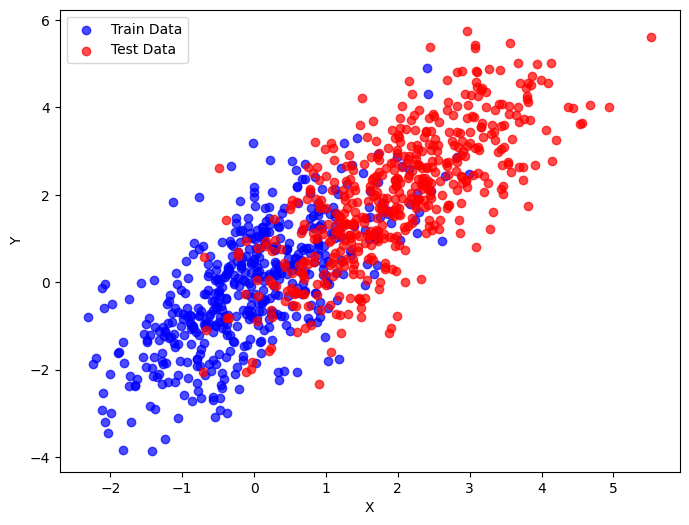
\includegraphics[width=0.7\textwidth]{images/Figure 0.png}
    \captionsetup{format=hang, singlelinecheck=false}
    \caption{Visual example of training data and test data drawn from Gaussian distribution with mean shift. Here, the training sample (in blue) are drawn from $\mathcal{N}(0,1)$ and the test sample (in red) are drawn from $\mathcal{N}(2, 1)$ each with a sample size of $500$ and the underlying relation: $y_i = x_i + \epsilon_i, \quad \epsilon_i \sim \mathcal{N}(0, 1), \quad i = 1, \ldots, 500$. This is just for visual example of how covariate shift effects and in our experiment, we are not working on this data.}
    \label{fig:0}
\end{figure}

\textbf{Measure of Performance}:\\

For our experiment, since we are focusing on linear regression, we have considered \textcolor{blue}{\emph{mean square error} (MSE)} as the \emph{loss function} to measure the error in predicting the outcome.\\

For an estimator $\hat{f}(x) = \langle \hat{\theta}, x \rangle$, the mean square error on a test sample $(\tilde{x}_i, \tilde{y}_i)$ is measured as:

\begin{equation}
    \text{MSE} = \frac{1}{n} \sum_{i=1}^n (\hat{f}(\tilde{x}_i) - \tilde{y}_i)^2 = \frac{1}{n} \sum_{i=1}^n \left( \langle \hat{\theta}, \tilde{x}_i \rangle - \tilde{y}_i \right)^2
    \label{eqn:6.2}
\end{equation}

i.e., the average squared difference between the true value and predicted value of the outcome, where $n$ is the number of samples in the test dataset.

\section{Effect of Mean Shift on MSE}

Now, we experiment how the mean shift $\mu$ affect the model performance in estimating the outcome using two most popular methods: \textcolor{blue}{\emph{Ordinary Least Square (OLS)}} and \textcolor{blue}{\emph{Gradient Descent}}.

\subsection{Ordinary Least Square (OLS) Estimator}

We briefly recall the definition of OLS for a \emph{design matrix} $\mathbf{X} \in \mathbb{R}^{n \times d}$ below.

\begin{definition}[Ordinary Least Squares]
When the design matrix $\mathbf{X}$ has full column rank, i.e., $\text{rank}(\mathbf{X}) = d$ meaning, the problem is \emph{overdetermined} and we have $n \geq d$ (more observations than feature dimensions), then the minimizer of the empirical risk (with least sqaure loss function)

\begin{equation}
    \mathcal{R}(\theta) = \frac{1}{n} \lVert \mathbf{Y} - \mathbf{X}\theta \rVert_2^2
    \label{eqn:6.3}
\end{equation}

is as below:

\begin{equation}
    \hat{\theta}_{\text{OLS}} := \argmin_{\theta \in \mathbb{R}} \mathcal{R}(\theta) = \argmin_{\theta \in \mathbb{R}} \frac{1}{n} \lVert \mathbf{Y} - \mathbf{X}\theta \rVert_2^2
    \label{eqn:6.4}
\end{equation}

and is called the \emph{Ordinary Least Squares} estimator.
\end{definition}

\begin{proposition}[Closed form solution of OLS]
If $\text{rank}(\mathbf{X}) = d$, we can show that $\hat{\theta}_{\text{OLS}}$ exists and is unique. It also attains a closed form solution \citep{aitken1936least, rao1945information}:

\begin{equation}
    \hat{\theta}_{\text{OLS}} = (\mathbf{X}^\top \mathbf{X})^{-1}\mathbf{X}^\top \mathbf{Y}
    \label{eqn:6.5}
\end{equation}
\end{proposition}

In our problem setting, we use this closed form solution to estimate the parameter $\theta$ and use them to predict the outcome for inputs $\tilde{x}$ from test dataset $\mathcal{T}_{\mu}$ for varying $\mu$. Finally, we measure our performance by calculating MSE and plot the resulting MSE against the corresponding mean shift ($\mu$).

\begin{figure}[h!]
    \centering
    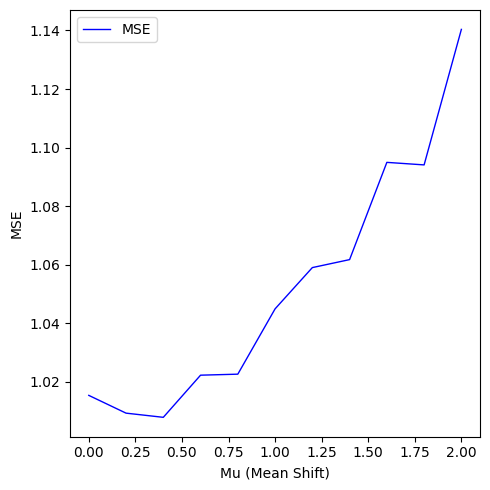
\includegraphics[width=0.5\textwidth]{images/Figure 1.png}
    \captionsetup{format=hang, singlelinecheck=false}
    \caption{Effect of varying mean shift on Mean Square Error (MSE) in Ordinary Least Square (OLS) estimator setup}
    \label{fig:1}
\end{figure}

Figure \ref{fig:1} illustrates the effect of covariate shift on model performance using ordinary least squares (OLS) estimator. As the mean shift ($\mu$) increases, the MSE also rises, indicating that the model's predictive accuracy deteriorates when the input distribution (test data) deviates from its training distribution. Initially, small shifts ($\mu < 0.5$) have a minor impact, but as $\mu$ grows, the error escalates more rapidly, suggesting a significant sensitivity to distributional changes. This behavior highlights the challenges posed by covariate shift.\\

\subsection{Gradient Descent Estimator}

Now, we will repeat the experiment with Gradient Descent with two different step size, $\gamma = 0.1$ and $\gamma=0.05$, to also observe the effect of step size ($\gamma$) on convergence rate. We recall the definition gradient descent before.

\begin{definition}[Gradient Descent]
The gradient descent is an iterative method where in each iteration, it moves towards the direction of steepest descent to move closer to the minima \citep{cauchy1847gradient}. It iterates with fixed step size $\gamma > 0$ and an initial parameter $\theta_0 \in \mathbb{R}^d$.\\

For a empirical risk with least-square loss function
\begin{equation}
    \mathcal{R}(\theta) = \frac{1}{n} \lVert \mathbf{Y} - \mathbf{X}\theta \rVert_2^2
    \label{eqn:6.6}
\end{equation}
the gradient is given by

\begin{equation}
    \begin{aligned}
        \nabla \hat{\mathcal{R}}(\theta) &= \frac{2}{n} \mathbf{X}^\top (\mathbf{X}\theta - \mathbf{Y})\\
        &= \frac{2}{n} \mathbf{X}^\top\mathbf{X}\theta - \frac{2}{n} \mathbf{X}^\top\mathbf{Y}
    \end{aligned}
    \label{eqn:6.7}
\end{equation}

and the estimated parameter $\hat{\theta}$ after $t+1$ iterations is given by
\begin{equation}
    \begin{aligned}
        \hat{\theta}_{t+1} &= \hat{\theta}_t - \gamma \nabla \hat{\mathcal{R}}(\hat{\theta}_t)\\
        &= (\mathbf{I}_d - 2 \frac{\gamma}{n}\mathbf{X}^\top \mathbf{X})\hat{\theta}_t + 2 \frac{\gamma}{n} \mathbf{X}^\top \mathbf{Y}
    \end{aligned}
    \label{eqn:6.8}
\end{equation}

\end{definition}

\begin{figure}[h!]
    \centering
    \begin{subfigure}{\textwidth}
        \centering
        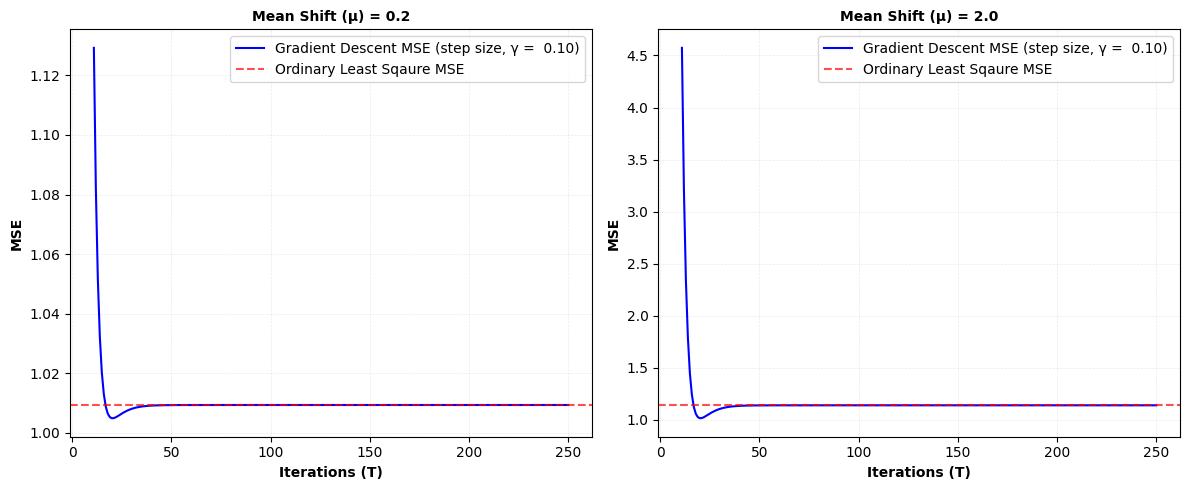
\includegraphics[width=\linewidth]{images/Figure 2a.png}
        \caption{Step size, $\gamma = 0.1$}
        \label{fig:2a}
    \end{subfigure}
    \hfill
    \begin{subfigure}{\textwidth}
        \centering
        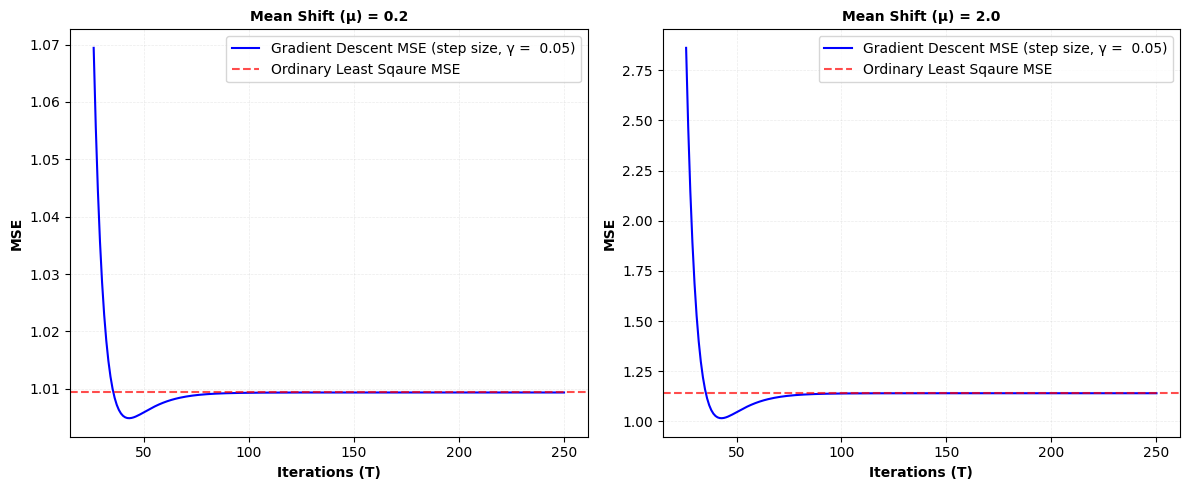
\includegraphics[width=\linewidth]{images/Figure 2b.png}
        \caption{Step size, $\gamma = 0.05$}
        \label{fig:2b}
    \end{subfigure}
    \captionsetup{format=hang, singlelinecheck=false}
    \caption{The image on left side plots the MSE against the increasing iterations for a mean shift, $\mu = 0.2$. The image on the right shows the same experiment for $\mu = 2.0$. We have chosen two extreme mean shift values to show the extreme effects. The experiment was carried out for two different step size, \textbf{(a)} $\gamma = 0.1$ and \textbf{(b)} $\gamma = 0.05$, to also observe the effect of step size ($\gamma$) on the convergence rate. \textbf{Note}: For better visualization purpose, the number of iterations on X-axis are truncated (initial few iterations are removed) in all plots to show the dip in curve prominently.}
    \label{fig:2}
\end{figure}

In our problem setting, we use $\theta_0 = \boldsymbol{0}^{10}$ (a vector of zero) and run the estimator for $250$ iterations, i.e., $\text{T}_{\text{max}} = 250$. We carry out the experiment using gradient descent for two different step sizes, $\gamma=0.1$ and $\gamma=0.05$.\\

Figure \ref{fig:2} illustrates the behavior of Mean Squared Error (MSE) using gradient descent method under different levels of covariate shift ($\mu = 0.2$ in left and $\mu = 2.0$ in right) and different step sizes, $\gamma=0.1$ in top and $\gamma=0.05$ in bottom. We observe that for gradient descent, the MSE initially starts at a high value and decreases rapidly as iterations increase, indicating convergence towards a minimum. However, for $\mu = 2.0$ (right), the initial MSE is significantly higher compared to $\mu = 0.2$ (left), suggesting that greater distribution shifts lead to higher initial errors. This behavior is observed for both step sizes and can be seen more precisely seen for all the mean shift ($\mu$) values in Figure \ref{fig:3}.\\

From Figure \ref{fig:2}, we also observe that irrespective of the choice of the step size ($\gamma$) and mean shift ($\mu$), the MSE dips below the OLS baseline before eventually converging towards it, implying that iterative optimization can momentarily outperform OLS but ultimately stabilizes around a similar error level. However, the convergence rate depends on the step size ($\gamma$), with higher $\gamma$ helps in converging faster. This can be observed in Figure \ref{fig:2a}, where the gradient descent with $\gamma=0.1$ converges to the OLS baseline in $\sim 40$ iterations, whereas it takes $\sim 80$ iterations with $\gamma=0.05$ (Figure \ref{fig:2b}).\\

Overall, the results from Figure \ref{fig:2} highlight the impact of covariate shift on learning dynamics, where larger shifts exacerbate the initial error but do not necessarily affect the final convergence behavior. Also, the choice of step size ($\gamma$) affects the convergence rate to a great extent. Since our main goal is to minimize the MSE as much as possible, so if we can select an \textcolor{blue}{\emph{optimal stopping time}} ($\text{T}_{\text{opt}}$), then gradient descent estimator will give us a better result than the baseline of ordinary least squares estimator.\\

By theory, the bias in expected excess risk decreases with the number of iterations, while the variance in expeced excess risk increases. At optimal stopping time ($\text{T}_{\text{opt}}$), we achieve a balance between these two (both becomes equal) and we found an upper bound of expected excess risk.

\begin{proposition}[Optimal Stopping Time and Upper Bound of Expected Excess Risk]
Choosing
\begin{equation}
    \text{T}_{\text{opt}} = \frac{\sqrt{n}\lVert \theta^* \rVert}{\gamma \sigma \sqrt{2 \text{ Trace}[\hat{\Sigma}]}},
    \label{eqn:6.9}
\end{equation}

the expected excess risk satisfies
\begin{equation}
    \mathbb{E}[\mathcal{R}(\hat{\theta}_{\text{T}_{\text{opt}}})] - \mathcal{R}^* \leq \frac{4\sigma \lVert \theta^* \rVert \text{ Trace}[\hat{\Sigma}]^{\frac{1}{2}}}{\sqrt{n}}
    \label{eqn:6.10}
\end{equation}

where $n$ is the sample size, $\sigma$ is the standard deviation in the noise $\epsilon$ and $\hat{\Sigma} = \frac{1}{n} \mathbf{X}^\top \mathbf{X}$ is the covariance matrix.
\end{proposition}

\begin{figure}[h!]
    \centering
    \begin{subfigure}{0.49\textwidth}
        \centering
        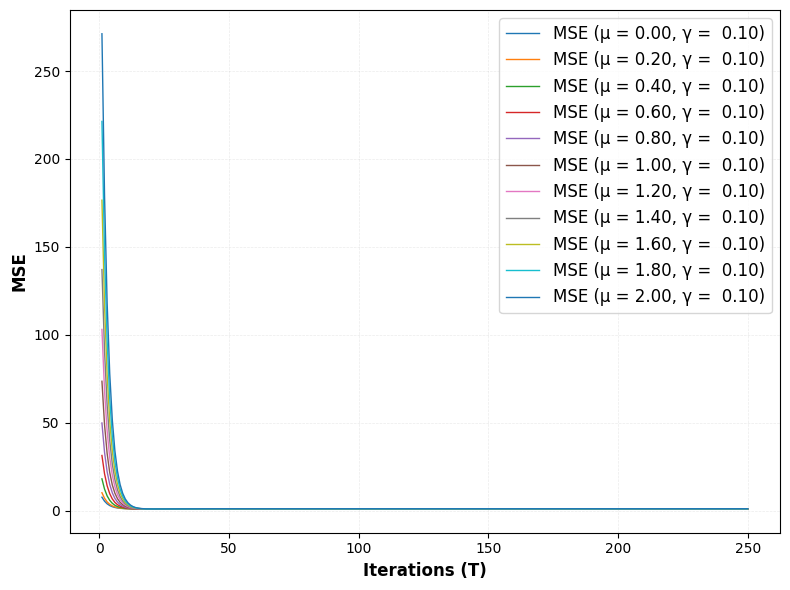
\includegraphics[width=\linewidth]{images/Figure 3a.png}
        \caption{Step size, $\gamma = 0.1$}
        \label{fig:3a}
    \end{subfigure}
    \hfill
    \begin{subfigure}{0.49\textwidth}
        \centering
        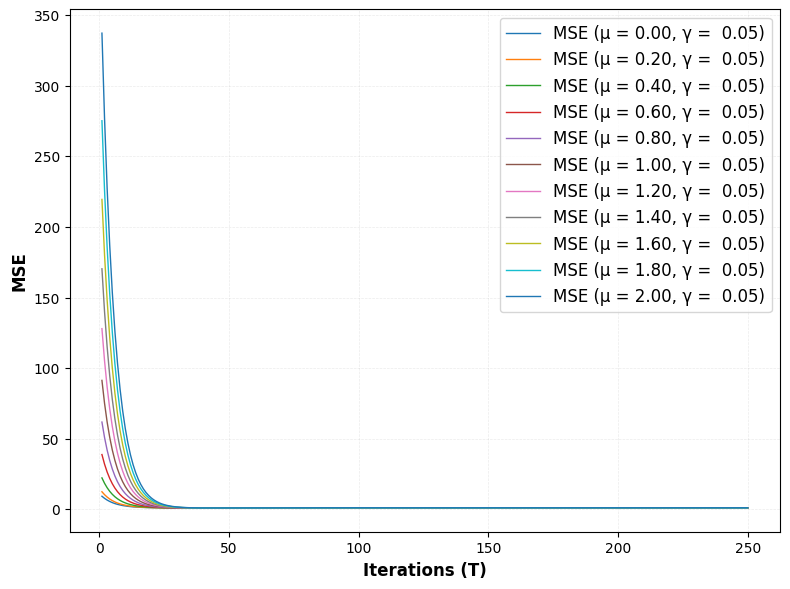
\includegraphics[width=\linewidth]{images/Figure 3b.png}
        \caption{Step size, $\gamma = 0.05$}
        \label{fig:3b}
    \end{subfigure}
    \captionsetup{format=hang, singlelinecheck=false}
    \caption{Initial value and rapid change in MSE with increasing iterations for multiple mean shifts, $\mu$. With a higher $\mu$, the initial value of MSE is greater compared to that with lower $\mu$. Also, with \textbf{(a)} higher step size ($\gamma = 0.1$), gradient descent converges much faster than gradient descent with \textbf{(b)} lower step size ($\gamma = 0.05$).}
    \label{fig:3}
\end{figure}

Figure \ref{fig:4} shows, more prominently using a heatmap, what we already observed before. A lower value of $\mu$ results in a much greater MSE initially as compared to the MSE for a higher $\mu$. As one can expect, for higher mean shift ($\mu$), it also takes longer iterations for the gradient descent to converge and reach minimum. The convergence rate also depends on the step size ($\gamma$): a higher step size ($\gamma = 0.1$) (Figure \ref{fig:4a}) achieves faster convergence than a lower step size ($\gamma = 0.05$) (Figure \ref{fig:4b}).\\

\begin{figure}[h!]
    \centering
    \begin{subfigure}{0.49\textwidth}
        \centering
        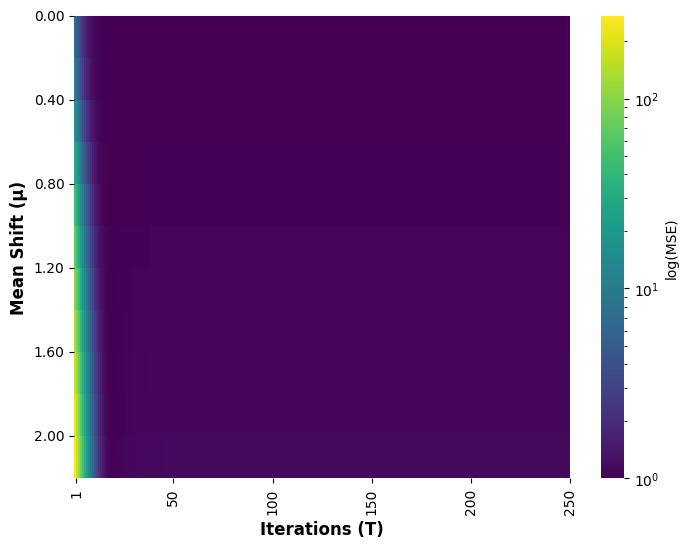
\includegraphics[width=\linewidth]{images/Figure 4a.png}
        \caption{Step size, $\gamma = 0.1$}
        \label{fig:4a}
    \end{subfigure}
    \hfill
    \begin{subfigure}{0.49\textwidth}
        \centering
        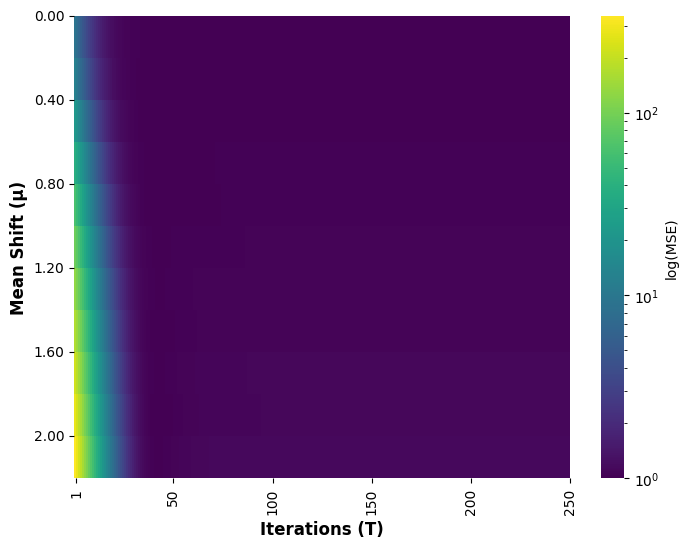
\includegraphics[width=\linewidth]{images/Figure 4b.png}
        \caption{Step size, $\gamma = 0.05$}
        \label{fig:4b}
    \end{subfigure}
    \captionsetup{format=hang, singlelinecheck=false}
    \caption{Heatmap of MSE to compare mean shift ($\mu$), iterations ($\text{T}$) and MSE in a single plot. Higher mean shift results in greater MSE initially and naturally it takes longer iterations for the gradient descent to minimize the MSE. Results are illustrated with \textbf{(a)} $\gamma = 0.1$ and \textbf{(b)} $\gamma = 0.05$. The logarithm of MSE is taken in the color bar for better scaling.}
    \label{fig:4}
\end{figure}


\begin{figure}[h!]
    \centering
    \begin{subfigure}{0.6\textwidth}
        \centering
        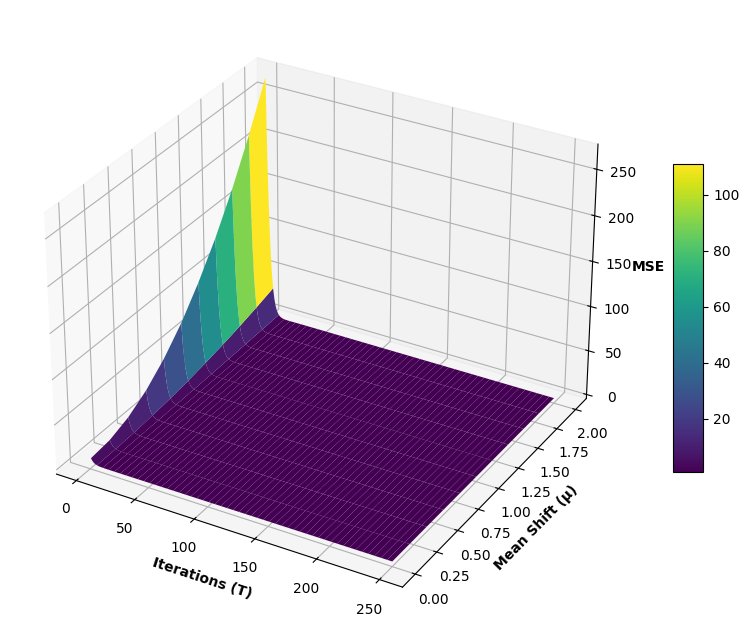
\includegraphics[width=\linewidth]{images/Figure 8a.png}
        \caption{Step size, $\gamma = 0.1$}
        \label{fig:5a}
    \end{subfigure}
    \hfill
    \begin{subfigure}{0.6\textwidth}
        \centering
        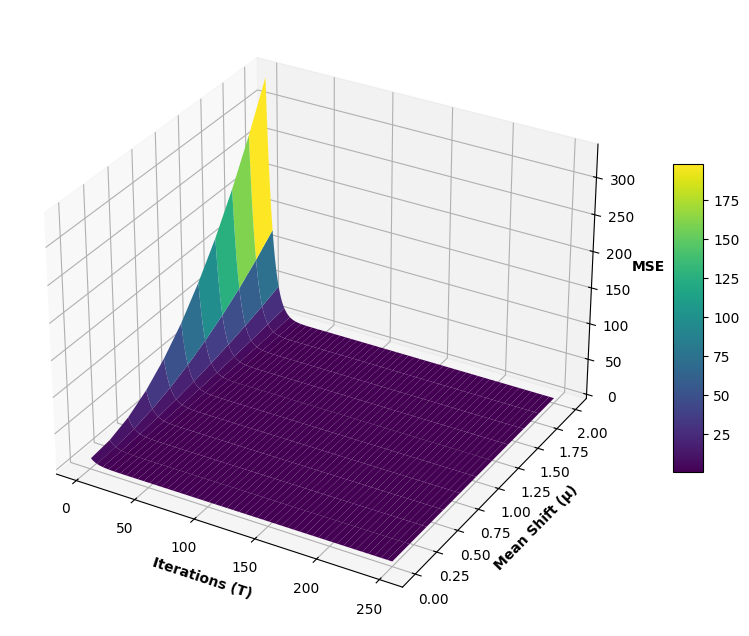
\includegraphics[width=\linewidth]{images/Figure 8b.png}
        \caption{Step size, $\gamma = 0.05$}
        \label{fig:5b}
    \end{subfigure}
    \captionsetup{format=hang, singlelinecheck=false}
    \caption{$3$-dimensional surface plot of interplay among mean shift ($\mu$), iteration count ($\text{T}$) and the respective mean square error (MSE) value in gradient descent method. The experiment was run using both \textbf{(a)} step size, $\gamma = 0.1$ and \textbf{(b)} step size, $\gamma = 0.05$.}
    \label{fig:5}
\end{figure}

The 3D plot in Figure \ref{fig:5} again visualizes the relationship between MSE (Mean Squared Error), iteration count in gradient descent ($\text{T}$), and mean shift ($\mu$) using two different step sizes, $\gamma = 0.1$ and $\gamma = 0.05$. Both plot shows that for small values of $\mu$, the MSE remains relatively low and stable as iterations increase. However, for larger values of $\mu$, the initial MSE is significantly higher, indicating a stronger negative impact of distribution shift on model performance. As iterations progress, the MSE decreases and stabilizes, suggesting convergence. The steep rise at the beginning for large $\mu$ values highlights the sensitivity of the model to distributional changes.\\


\begin{figure}[h]
    \centering
    \begin{subfigure}{0.48\textwidth}
        \centering
        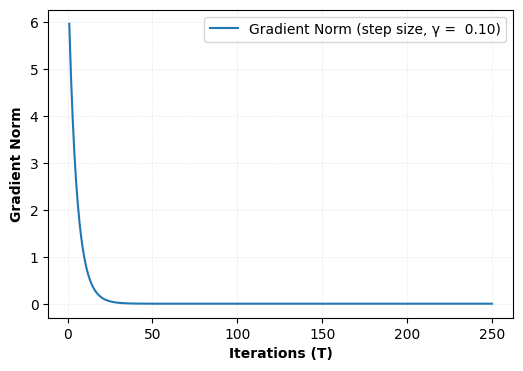
\includegraphics[width=\linewidth]{images/Figure 5a.png}
        \caption{Step size, $\gamma = 0.1$}
        \label{fig:6a}
    \end{subfigure}
    \hfill
    \begin{subfigure}{0.48\textwidth}
        \centering
        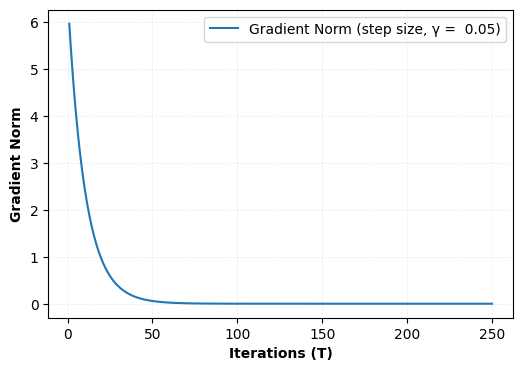
\includegraphics[width=\linewidth]{images/Figure 5b.png}
        \caption{Step size, $\gamma = 0.05$}
        \label{fig:6b}
    \end{subfigure}
    \hfill
    \begin{subfigure}{0.48\textwidth}
        \centering
        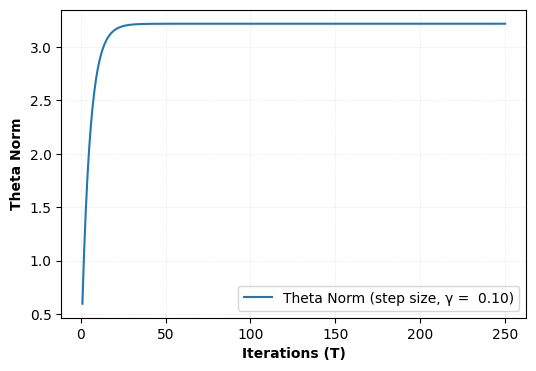
\includegraphics[width=\linewidth]{images/Figure 6a.png}
        \caption{Step size, $\gamma = 0.1$}
        \label{fig:6c}
    \end{subfigure}
    \hfill
    \begin{subfigure}{0.48\textwidth}
        \centering
        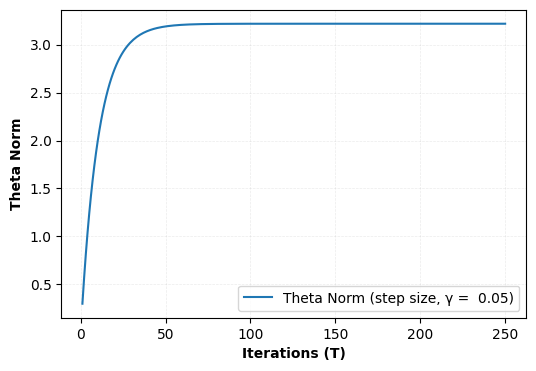
\includegraphics[width=\linewidth]{images/Figure 6b.png}
        \caption{Step size, $\gamma = 0.05$}
        \label{fig:6d}
    \end{subfigure}
    \captionsetup{format=hang, singlelinecheck=false}
    \caption{Illustration of how \textbf{(a)}, \textbf{(b)} the gradient norm $\lVert \nabla \hat{\mathcal{R}}(\theta) \rVert$ and \textbf{(c)}, \textbf{(d)} parameter norm $\lVert \hat{\theta}^{\text{GD}} \rVert$ change across iterations during the training using gradient descent method.}
    \label{fig:6}
\end{figure}

Figure \ref{fig:6} shows how the gradient norm $\lVert \nabla \hat{\mathcal{R}}(\theta) \rVert$ (Figure \ref{fig:6a} and Figure \ref{fig:6b}) and parameter norm $\lVert \hat{\theta}^{\text{GD}} \rVert$ (Figure \ref{fig:6c} and Figure \ref{fig:6d}) change during the gradient descent iterations. Since we learn the parameter only from the training sample $\mathcal{S} \sim \mathcal{N}(0, 1)$, this does not depend on the mean shift ($\mu$).\\

As we observe in Figure \ref{fig:6a} and \ref{fig:6b}, $\lVert \nabla \hat{\mathcal{R}}(\theta) \rVert$ initially starts with very high value and then with increasing iterations it steeply reduces, finally converging to $0$ in $\sim 30$ iterations for $\gamma=0.1$ and in $\sim 60$ iterations for $\gamma=0.05$. This is because the gradient norm measures how large the gradient is at a given point. A large gradient norm means the function is steep, and updates will be large, whereas, a small gradient norm means the function is flat, and updates will be small. At the beginning, the gradient norm is high because the parameters are far from the optimal values. As iterations progress, the optimizer moves downhill in the loss landscape, reducing both the loss and the gradient norm. Closer to the minimum, the gradient norm approaches zero because the function is nearly flat (stationary point).\\

The same logic explains the observations in Figure \ref{fig:6c} and \ref{fig:6d}. Initially, 
$\lVert \hat{\theta}^{\text{GD}} \rVert$, representing the norm (magnitude) of the parameter vector $\theta$, starts near zero. It rapidly increases within the first few iterations. The rate of increase slows down, and 
finally it plateaus at a final value around $\approx 3.2$ in $\sim 30$ and $\sim 60$ iterations respectively for $\gamma=0.1$ and $\gamma=0.05$. We recall that the parameters are updated in iterations by taking a step towards the gradient direction: $\hat{\theta}_{t+1} = \hat{\theta}_t - \gamma \nabla \hat{\mathcal{R}}(\hat{\theta}_t)$. At the beginning, gradient updates are large because the model parameters are far from optimal. As the optimizer updates $\theta$ through iterations, it moves towards an optimal region, causing the norm to increase. Eventually, closer to the minimum, the gradient approaches zero, meaning the parameters stabilize, and further updates are minimal.\\

Moreover, we also observe how it takes significantly less number of iterations for both the norms to reach its optimal value by increasing the step size from $\gamma=0.05$ to $\gamma=0.1$.



\subsection{Comparison between OLS and GD estimator (Effect of Mean Shift)}

We finally compare the performance from both ordinary least squares and gradient descent estimator (with different step sizes) for varying $\mu$ to observe the affect of mean shift on their performance.\\

\begin{figure}[h!]
    \centering
    \begin{subfigure}{\textwidth}
        \centering
        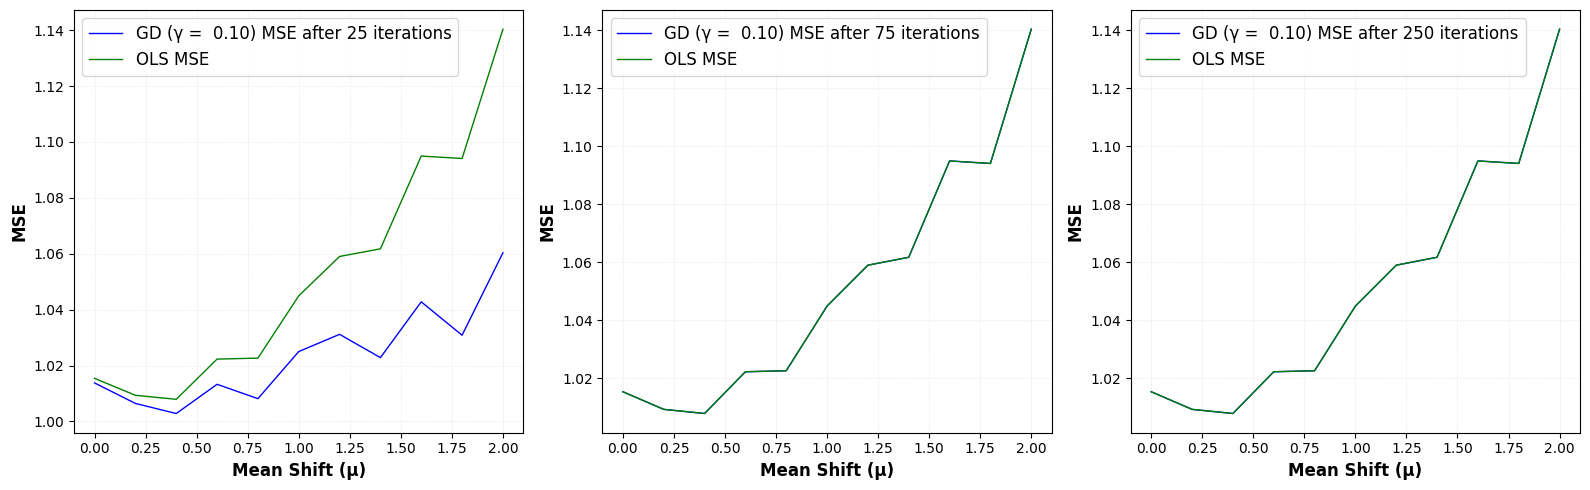
\includegraphics[width=\linewidth]{images/Figure 7a.png}
        \caption{Step size, $\gamma = 0.1$}
        \label{fig:7a}
    \end{subfigure}
    \hfill
    \begin{subfigure}{\textwidth}
        \centering
        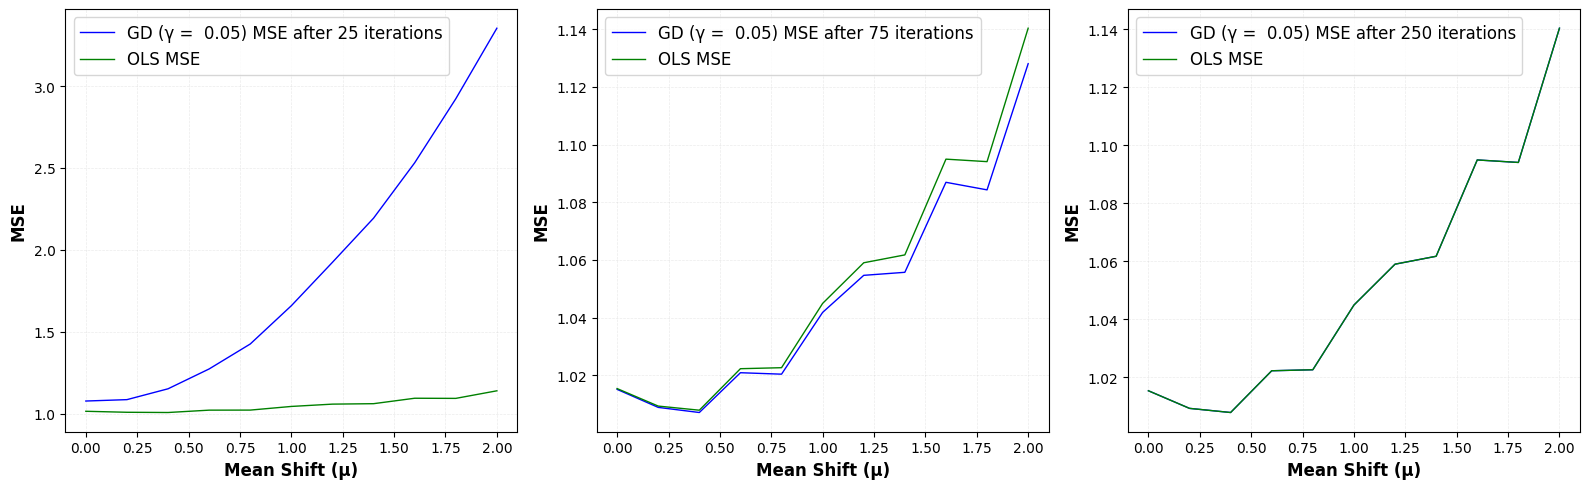
\includegraphics[width=\linewidth]{images/Figure 7b.png}
        \caption{Step size, $\gamma = 0.05$}
        \label{fig:7b}
    \end{subfigure}
    \captionsetup{format=hang, singlelinecheck=false}
    \caption{Mean Squared Error (MSE) of Gradient Descent (GD) and Ordinary Least Squares (OLS) as a function of Mean Shift ($\mu$), for different numbers of iterations ($\text{T}$): (I) results at $\text{T}=25$, (II) results at $\text{T} = 75$ and (III) results at $\text{T} = 250$. This is to observe the results during the beginning, after a few iterations and at the very end of the total iterations in gradient descent. The experiment is done twice for different step sizes: \textbf{(a)} $\gamma=0.1$ and \textbf{(b)} $\gamma=0.05$}
    \label{fig:7}
\end{figure}

The three-panel plot in Figure \ref{fig:7} plots the Mean Squared Error (MSE) obtained in Gradient Descent (GD) and Ordinary Least Squares (OLS) for different mean shift ($\mu$). We have plotted the result for three different iteration count ($\text{T}$): the leftmost plot corresponds to $\text{T}=25$, the middle plot to $\text{T} = 75$, and the rightmost plot to $\text{T}=250$. The three plots above (Figure \ref{fig:7a}) represents gradient descent with step size, $\gamma = 0.1$ while the three plots below (Figure \ref{fig:7b}) represents gradient descent with step size, $\gamma = 0.05$.\\

We can observe that initially at $\text{T}=25$, the GD MSE (blue) is significantly higher than the OLS MSE (green) for both values of $\gamma$, indicating that GD has not fully converged. Moreover, lower step size produces a smoother curve as the updates in each iterations are slower. As iterations increase to $\text{T} = 75$, the GD MSE with $\gamma = 0.05$ aligns almost closely with the OLS MSE, while the GD MSE with $\gamma = 0.1$ has already converged with the OLS MSE, suggesting better convergence. At $\text{T}=250$, GD and OLS produce identical errors, confirming that GD has converged to the optimal solution.\\

Additionally, across all plots, the MSE increases with $\mu$ for both gradient descent and OLS, indicating that a larger mean shift negatively impacts predictive accuracy. This behavior is expected since shifting the mean introduces distributional changes, making model estimation less effective. Overall, the results highlight that GD requires sufficient iterations to achieve optimal performance but can eventually approximate OLS solutions when properly tuned. The number of iterations also depends on the step size, $\gamma$.

\section{Regularizing Covariate Shift}

In the following section, we will try to regularize the affect mean shift ($\mu$) using importance weighting. We will use two different methods to estimate the weights: \emph{kernel density estimation} and \emph{self-attention mechanism}.

\subsection{Importance Weighting using Kernel Density Estimation}

As we recall from section \ref{imp-weight}, if $p_{\text{train}}(X)$ and $p_{\text{test}}(X)$ are the probability density functions of the input distribution $\mathbb{P}_{\text{train}}(X)$ and $\mathbb{P}_{\text{test}}(X)$ respectively, then the \textcolor{blue}{\emph{importance weights}} can be estimated as the ratio of test and training input densities at training input points:

\begin{equation}
    \omega(x_i) = \frac{p_{\text{test}}(x_i)}{p_{\text{train}}(x_i)}
    \label{eqn:6.11}
\end{equation}

$\mathbb{P}_{\text{train}}(X)$ and $\mathbb{P}_{\text{test}}(X)$ are also called \emph{source distribution} and \emph{target distribution} respectively.\\

In practical situations, we do not know which distribution is the training and test samples are drawn from. So the underlying probability density functions are also unknown. In such cases, we try to estimate the probability density function (PDF). One such method is \textcolor{blue}{\emph{Kernel Density Estimation}}.\\

\vspace{2em}
\textbf{Importance Weighted variant: Ordinary Least Square (OLS)}\\

We use the closed form solution in equation \ref{eqn:3.10} to compute the MSE in importance weighted setting using OLS estimator. For our experimental purpose, we have used \emph{Gaussian Kernel} to estimate the densities, as mentioned in equation \ref{eqn:3.5}.\\

Figure \ref{fig:9} compares the MSE calculated through standard OLS estimator (unweighted) and its importance weighted variant across varying mean shift ($\mu$). The comparison is done at different bandwidth level.\\

We recall that bandwidth controls the smoothness of the kernel density estimate. A smaller bandwidth produces a more detailed (possibly noisy) density estimate while a larger bandwidth produces a smoother density estimate, which might oversmooth the data and lose details. This behavior can be observed in Figure \ref{fig:9}. While with a smaller bandwidth, the estimated density is noisy (irregular), making the difference between MSE calculated for unweighted and weighted OLS greater and erratic. With a higher bandwidth ($h > 2.0$), the density becomes smoother and stable, hence the MSE of weighted OLS approaches towards the MSE of unweighted OLS. There might be even some loss of details contributing to this convergence.\\

We also observe in Figure \ref{fig:9} that the difference between MSE calculated for unweighted and weighted OLS increases with higher mean shift ($\mu$). This behavior is expected since shifting the mean introduces distributional changes, which results in the greater difference in respective MSE values.

\begin{figure}[h!]
    \centering
    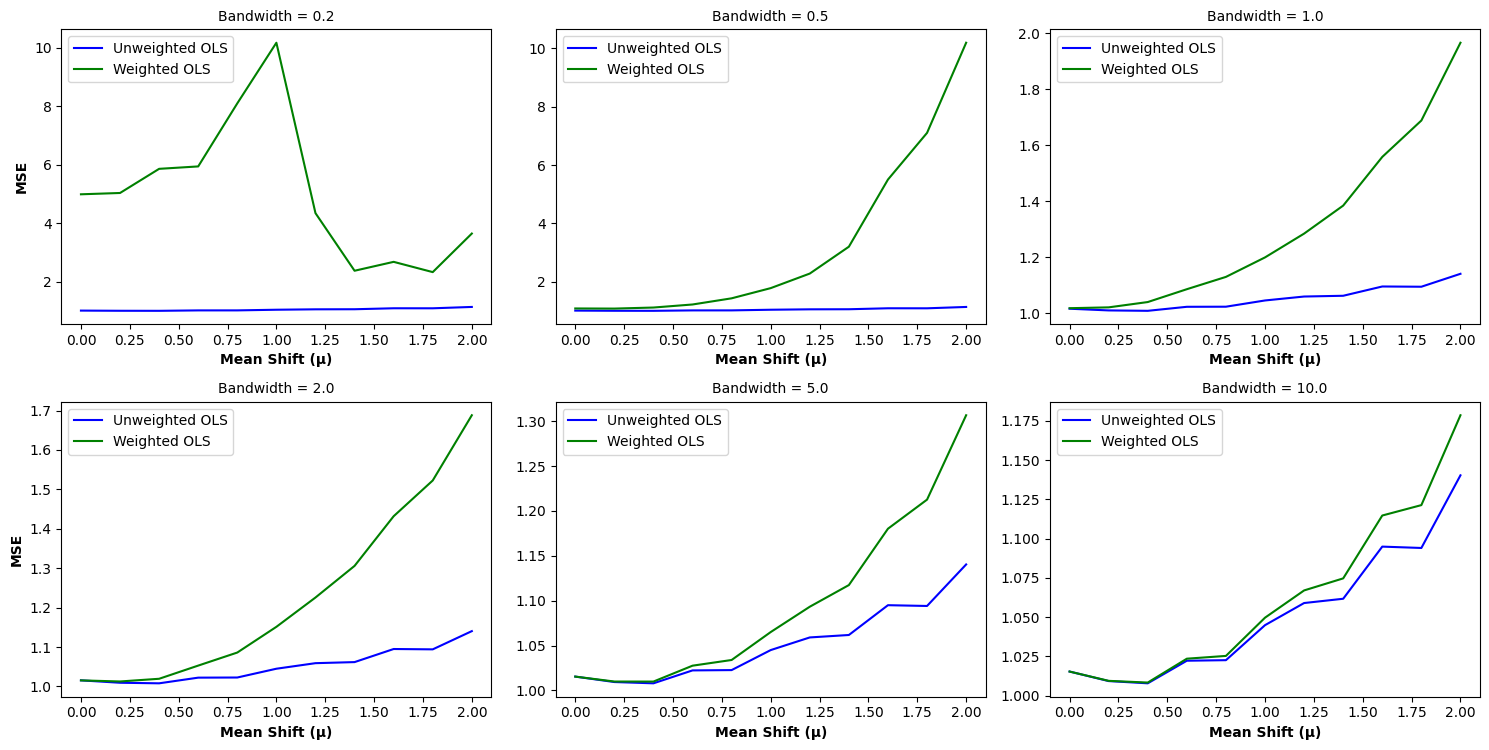
\includegraphics[width=\textwidth]{images/Figure 9.png}
    \captionsetup{format=hang, singlelinecheck=false}
    \caption{Effect of Importance Weighting (Kernel Density Estimation) with different bandwidth on MSE in Mean Shift setup. The MSE is calculated for both standard ordinary least square (unweighted) and importance weighted least square estimator at different bandwidth: (a) $h = 0.2$, (b) $h = 0.5$, (c) $h = 1.0$, (d) $h = 2.0$, (e) $h = 5.0$, (f) $h = 10.0$.}
    \label{fig:9}
\end{figure}

But even with the importance weighting, the regularization effect is not prominent since the MSE for weighted variant of OLS is consistently higher than that of unweighted variant (Figure \ref{fig:9}). This can have multiple reasons. To investigate further whether the sample size plays any role in the effect of mean shift on MSE, we plot the MSE for different sample sizes. At this moment, we \textbf{fix the mean shift} at $\mu = 1.0$ and use \textbf{fixed bandwidth} $=0.5$ (using \emph{Silverman's rule of thumb}: $h = 1.06 \times \sigma \times n^{-\frac{1}{5}}$, where $\sigma$ is the standard deviation of the data and $n$ is the sample size).

\begin{figure}[h!]
    \centering
    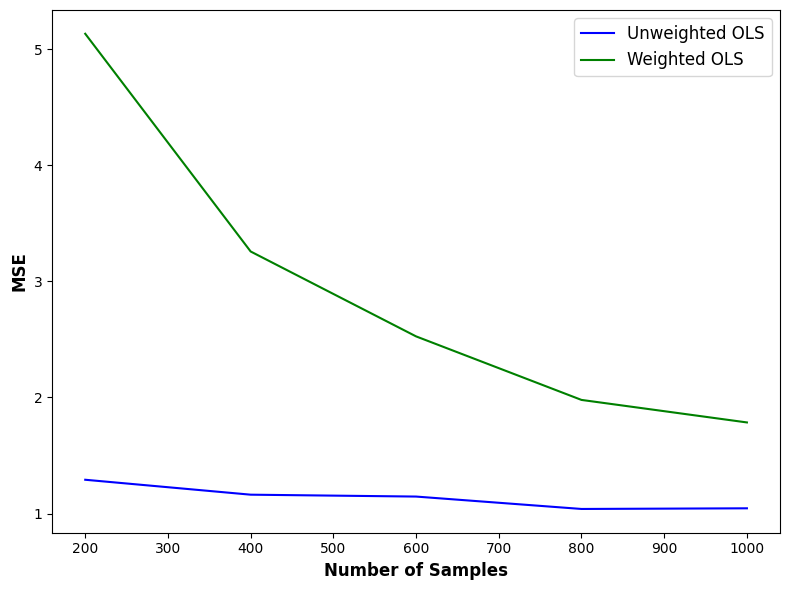
\includegraphics[width=0.7\textwidth]{images/Figure 10.png}
    \captionsetup{format=hang, singlelinecheck=false}
    \caption{Effect of sample size on mean shift regularization using importance weighting. The comparison is done between unweighted ordinary least square and importance weighted ordinary least square method at fixed mean shift ($\mu = 1.0$) and fixed bandwidth ($h=0.5$).}
    \label{fig:10}
\end{figure}

As we observe in Figure \ref{fig:10}, the sample size indeed plays a role. With higher sample sizes, the MSE calculated with weighted variant of OLS decreases rapidly and approaches the MSE of unweighted OLS. Due to limitation of computational resources, we couldn't experiment with any higher sample size, however this behavior is consistent with what we already discussed in section \ref{IWERM}, equation \ref{eqn:4.20}:
$$\lim_{n \to \infty} (\hat{\theta}_{\text{IWOLS}}) = \theta^*$$

Further investigation is required to investigate whether any other factors other than sample size plays a crucial role in regularizing the effect of mean shift by importance weighting.

\vspace{2em}
\textbf{Importance Weighted variant: Gradient Descent (GD)}\\

Similar to OLS, We use \ref{eqn:3.11} and \ref{eqn:3.12} to compute the MSE in importance weighted setting using OLS estimator. At this moment, we fix the mean shift at $\mu = 1.0$ and step size, $\gamma = 0.1$, bandwidth $= 0.5$ and increase the iteration count, $\text{T to } 5000$.\\

\begin{figure}[h!]
    \centering
    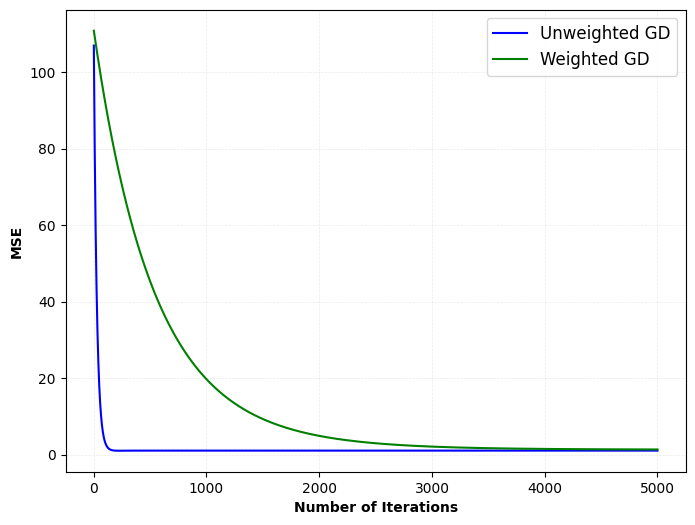
\includegraphics[width=0.6\textwidth]{images/Figure 11.png}
    \captionsetup{format=hang, singlelinecheck=false}
    \caption{Effect of importance weighting in mean shift regularization: Comparing MSE with unweighted and weighted variants of gradient descent, computed with step size, $\gamma = 0.1$ and iteration count, $\text{T} = 5000$. The experiment is done with fixed mean shift, $\mu = 1.0$ and bandwidth $= 0.5$.}
    \label{fig:11}
\end{figure}

Figure \ref{fig:11} shows the effect of importance weighting in regularizing the effect of mean shift by comparing the MSE calculated with both unweighted and weighted variants of gradient descent method. We observe here that with increasing iterations, the MSE calculated with weighted version of gradient descent is reducing steadily and approaching towards the MSE calculated with unweighted version of gradient descent, finally converging in $\sim 4000$ iterations. It was observed during the experiment that step size ($\gamma$) plays a crucial role, reducing it will take significantly more number of iterations to converge.\\

Once again, we try to investigate whether sample size plays any role in regularizing effect. As we observe in Figure \ref{fig:12}, increasing the sample size helps in regularizing the effect of mean shift. Keeping the number of iterations fixed at $\text{T} = 5000$, we can see that as sample size increases, performance of weighted gradient descent steadily approaches towards that of unweighted version and \emph{almost} converges with $1000$ sample sizes. Working with further sample size will require more computational resources.

\begin{figure}[h!]
    \centering
    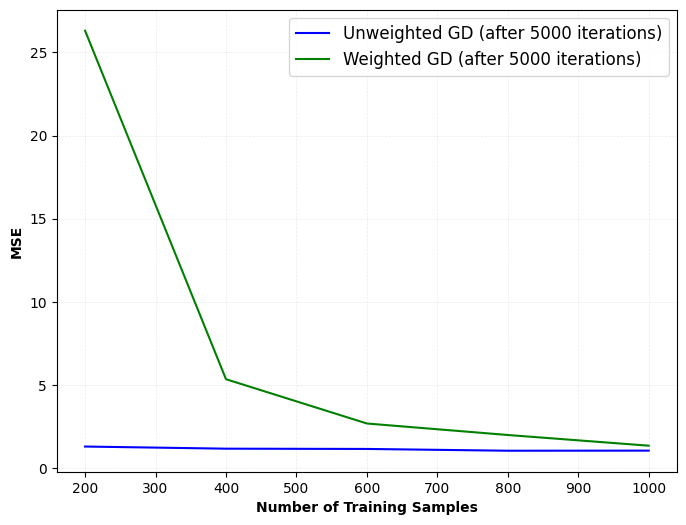
\includegraphics[width=0.5\textwidth]{images/Figure 12.png}
    \captionsetup{format=hang, singlelinecheck=false}
    \caption{Effect of sample size on regularizing mean shift by importance weighted gradient descent with $\text{T} = 5000$ iterations, step size, $\gamma = 0.1$ and sample size $=1000$.}
    \label{fig:12}
\end{figure}

In Figure \ref{fig:13}, we compare the performance of weighted OLS and weighted GD estimator, with a step size, $\gamma = 0.1$. We can observe here that unlike in the unweighted setup (Figure \ref{fig:2}), in the weighted setup, the gradient descent converges to OLS very steadily even with the same step size. It takes significantly higher number of iterations to converge to OLS compared to unweighted setup.\\

\begin{figure}[h!]
    \centering
    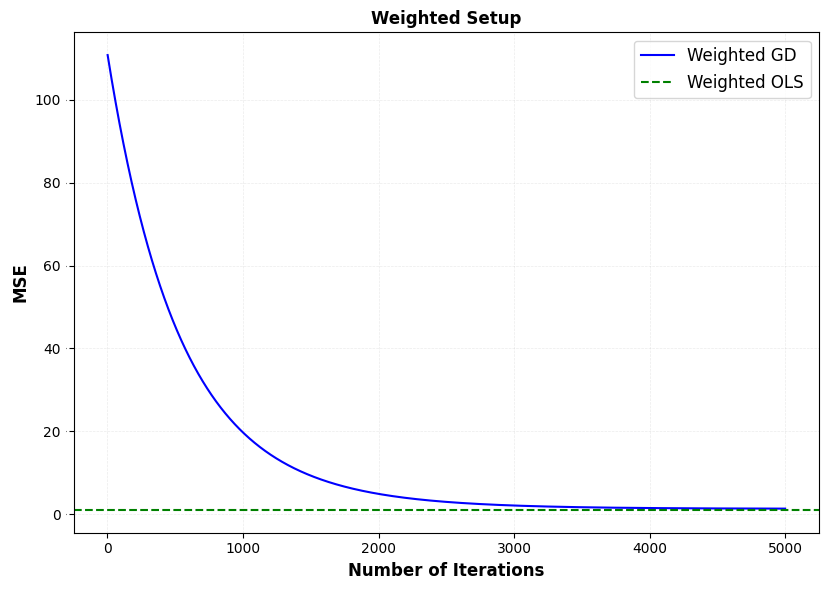
\includegraphics[width=0.6\textwidth]{images/Figure 13.png}
    \captionsetup{format=hang, singlelinecheck=false}
    \caption{Comparison of weighted OLS and weighted GD (step size, $\gamma = 0.1$) performance across iterations for fixed mean shift, $\mu = 1.0$.}
    \label{fig:13}
\end{figure}

One of the reason for this erratic behavior is of course is the sample size, as we have already established. Figure \ref{fig:14} shows the effect of sample size on regularizing mean shift by importance weighted variants of both OLS and gradient descent. Here we again compare the performance of gradient descent with that of OLS, in both weighted and unweighted setup, but in terms of sample size while keeping the iteration count fixed at $\text{T} = 5000$. This is in contrast to Figure \ref{fig:13}, where we had kept the sample size constant at $n = 1000$ and measured the performance against varying iteration count, $\text{T}$, in weighted setup.

\begin{figure}[h!]
    \centering
    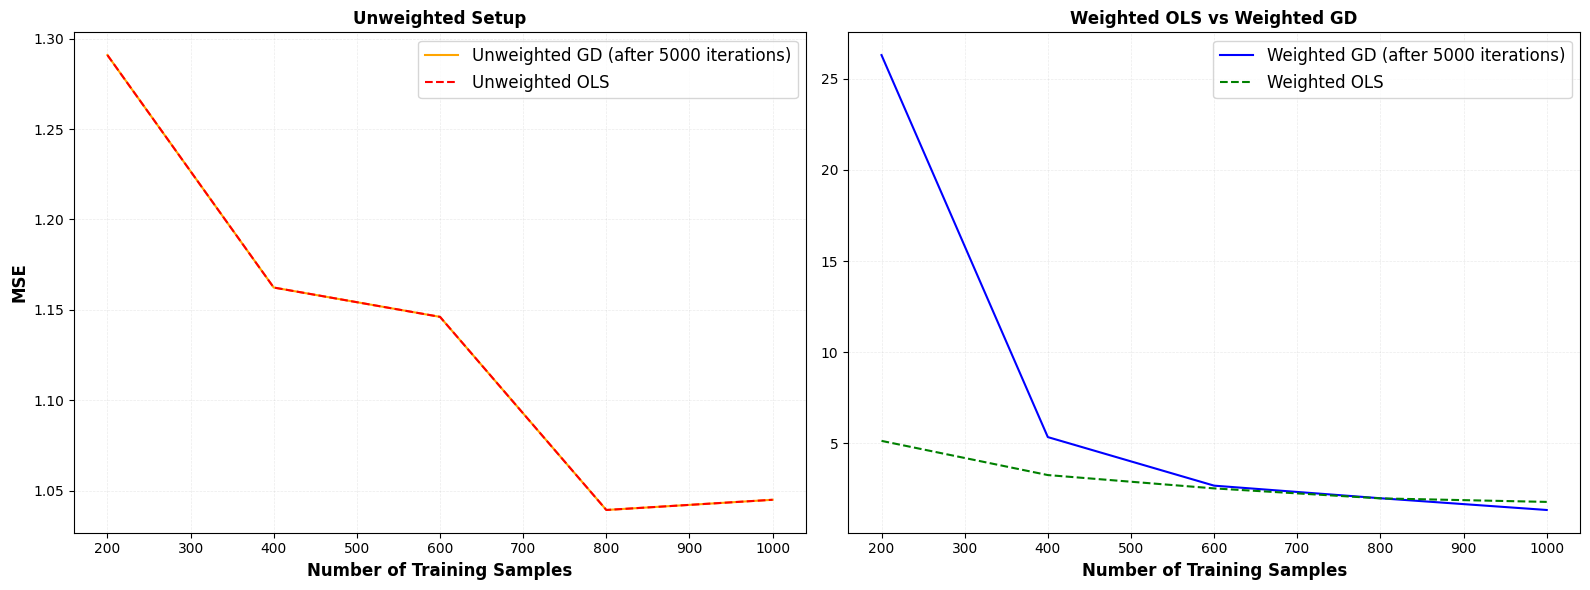
\includegraphics[width=\textwidth]{images/Figure 14.png}
    \captionsetup{format=hang, singlelinecheck=false}
    \caption{Effect of sample size on performance of OLS and gradient descent with step size, $\gamma=0.1$ after $\text{T} = 5000$ iterations in both weighted and unweighted setup.}
    \label{fig:14}
\end{figure}

Our observation from Figure \ref{fig:14} solidifies our learning so far that sample size plays a crucial role in importance weighting. For same number of iterations, the performance of importance weighted gradient descent and convergence with importance weighted OLS depends on the sample size. In our current setup, with $\sim 600$ samples the weighted gradient descent could converge to weighted OLS performance and with even higher sample size ($> 900$), the weighted gradient descent could even beat the performance of weighted OLS.\\

We should also note that in the unweighted setup as well, the performance of gradient descent depends on the sample size. This can be observed in Figure \ref{fig:15}. This is same as the previous figure, but the results are plotted after $\text{T} = 400$ iterations.

\begin{figure}[h!]
    \centering
    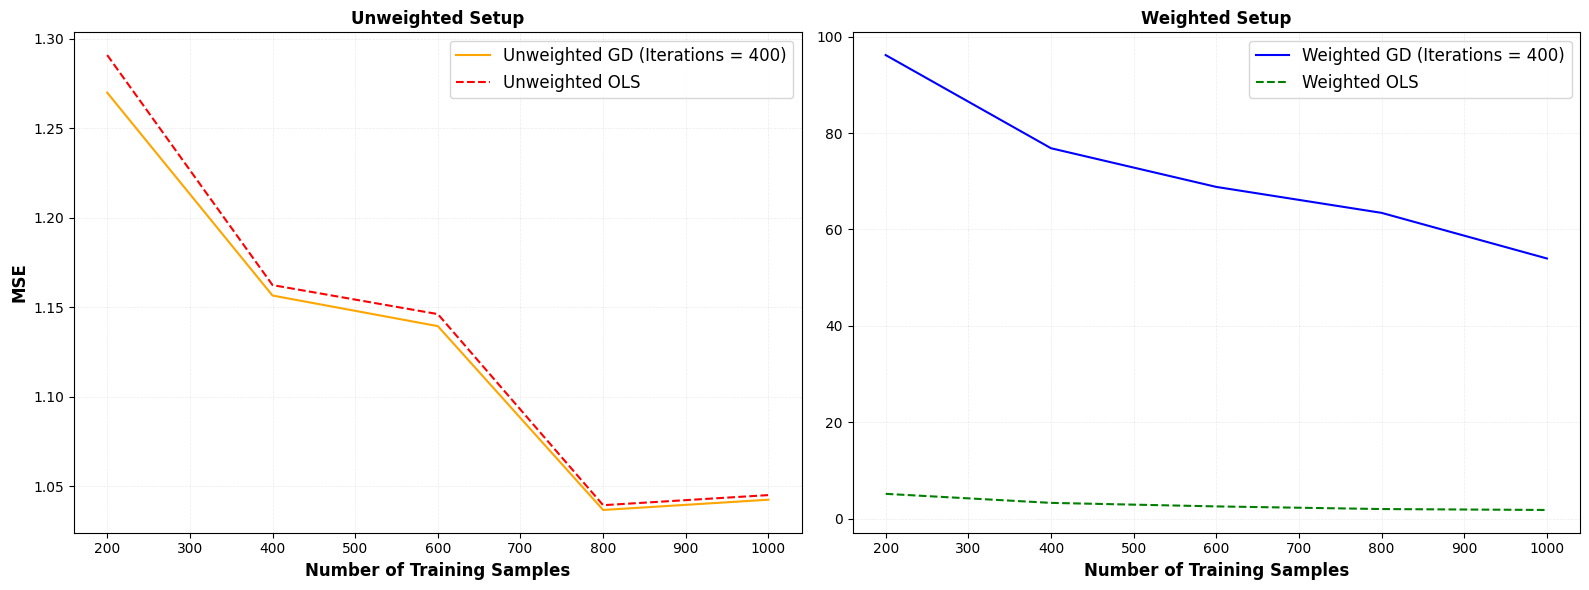
\includegraphics[width=\textwidth]{images/Figure 15.png}
    \captionsetup{format=hang, singlelinecheck=false}
    \caption{Effect of sample size on performance of OLS and gradient descent with step size, $\gamma=0.1$ after $\text{T} = 400$ iterations in both weighted and unweighted setup.}
    \label{fig:15}
\end{figure}

We can observe that in unweighted setup, even with a relatively low iteration of $\text{T} = 400$, a fairly lower sample size is enough for the performance of gradient descent to converge with that of OLS estimator. With higher iterations, even lower sample size can be enough for the convergence. 

\subsection{Self-attention Mechanism}

We recall from section \ref{self-attention} that for an empirical loss

\begin{equation}
    \hat{\mathcal{R}}(\theta, \omega) := \frac{1}{n} \sum_{i=1}^n m(\omega^{(i)})\ell (y_i, \langle \theta, x_i \rangle)
    \label{eqn:21}
\end{equation}

where $\omega = (\omega^{(1)}, \ldots, \omega^{(n)})$ is the importance weights and $m: \mathbb{R} \to \mathbb{R}$ is a masking function, the \textcolor{blue}{\emph{gradient descent-ascent algorithm}} with initial regression parameter, $\theta_0 = 0$ and initial weights, $\omega^{(i)}_0$ for all $i = 1, \ldots, n$ is given by:

\begin{equation}
    \begin{aligned}
        \theta_{t+1} &= \theta_t - \gamma_t \nabla_{\theta} \hat{\mathcal{R}}(\theta_t, \omega_t)\\
        \omega_{t+1} &= \omega_t - \eta_t \nabla_{\omega} \hat{\mathcal{R}}(\theta_t, \omega_t)
    \end{aligned}
    \label{eqn:6.12}
\end{equation}

where $\gamma_t$ and $\eta_t$ are the learning rates.\\

We compute the gradients of the above empirical risk with respect to $\omega$ and $\theta$ by:\\

\begin{equation}
    \begin{aligned}
        \nabla_{\theta}\hat{\mathcal{R}}(\theta, \omega) &= \frac{2}{n}\mathbf{X}^\top\mathbf{M}(\mathbf{X}\theta - \mathbf{Y})\\
        \nabla_{\omega}\hat{\mathcal{R}}(\theta, \omega) &= \frac{1}{n} \frac{dM(\omega)}{d\omega} (\mathbf{X}\theta - \mathbf{Y}) \odot (\mathbf{X}\theta - \mathbf{Y})
    \end{aligned}
    \label{eqn:6.13}
\end{equation}\\

For our experimental purpose, we have kept the step size, $\gamma = 0.1$ and iteration count, $\text{T} = 7500$ for the gradient descent-ascent algorithm. The experiment was carried out at a fixed mean shift, $\mu = 1.0$.\\

Figure \ref{fig:16} shows the effect of masking function is regularizing mean shift. The comparison involves unweighted gradient descent (GD) and weighted GD with Self-Attention-based Masking, using different masking strategies. As we recall from the definition \ref{masking} of masking function, using $q=0$ in the unbounded masking function $m_q(t) = t^q$ gives us unweighted variant, as $q=0$ ignores the effect of weighting.\\

\begin{figure}[h!]
    \centering
    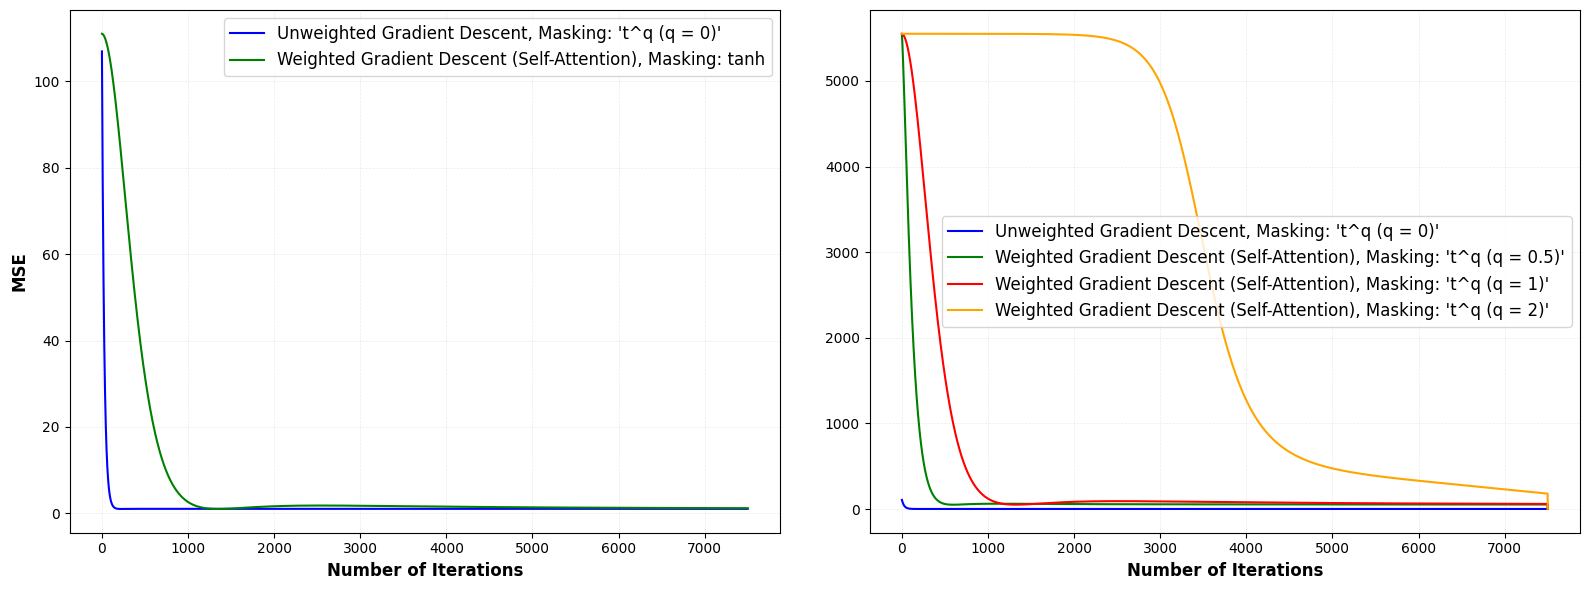
\includegraphics[width=\textwidth]{images/Figure 16.png}
    \captionsetup{format=hang, singlelinecheck=false}
    \caption{Regularizing mean shift by importance weighting using self-attention mechanism. The gradient descent-ascent algorithm was carried out at step size, $\gamma = 0.1$ and for $7500$ iterations. Left: uses $m(t) = tanh(t)$ masking function (bounded). Right: uses $m_q(t) = t^q$ masking function (unbounded) for $q \in [0.5, 1, 2]$.}
    \label{fig:16}
\end{figure}

The left subplot in Figure \ref{fig:16} uses a bounded masking function $m(t) = tanh(t)$. Both unweighted and weighted gradient descent methods exhibit a sharp initial drop in MSE, indicating rapid convergence. After a certain number of iterations ($\sim 1000$), both methods stabilize, reaching nearly the same final MSE. Also, the weighted GD initially decreases slower compared to unweighted GD but eventually reaches similar performance.\\

The right subplot in Figure \ref{fig:16} uses an unbounded masking function $m_q(t) = t^q$ and plots for different values of $q \in [0.5, 1, 2]$. We can observe that for smaller values of $q (=0.5)$, weighted gradient descent converges comparatively faster. However, for larger values of $q$ ($q = 2$), the initial MSE is extremely high, and convergence is much slower, possibly due to overemphasis on certain data points, leading to instability before gradually decreasing. This suggests that \emph{larger $q$ values in the self-attention weighting mechanism can lead to unstable learning process resulting in poor initial performance and slow adaptation}. This behavior aligns with our theoretical expectation from choosing high $q$ value in unbounded masking function $m_q(t) = t^q$, which we discussed in section \ref{choice-masking-q} (Choice of Masking Function).\\

Overall, we also observe from Figure \ref{fig:16} that the initial MSE for bounded masking function $m(t) = tanh(t)$ is much lower than the unbounded masking function $m_q(t) = t^q$. It can also be noted that the unbounded masking function with $q=1$ takes almost same number of iterations to converge to the unweighted gradient descent MSE as the bounded masking function.\\

We also want to see how sample size plays a role in the choice of masking function during the importance weighting with self-attention mechanism. 

\begin{figure}[h!]
    \centering
    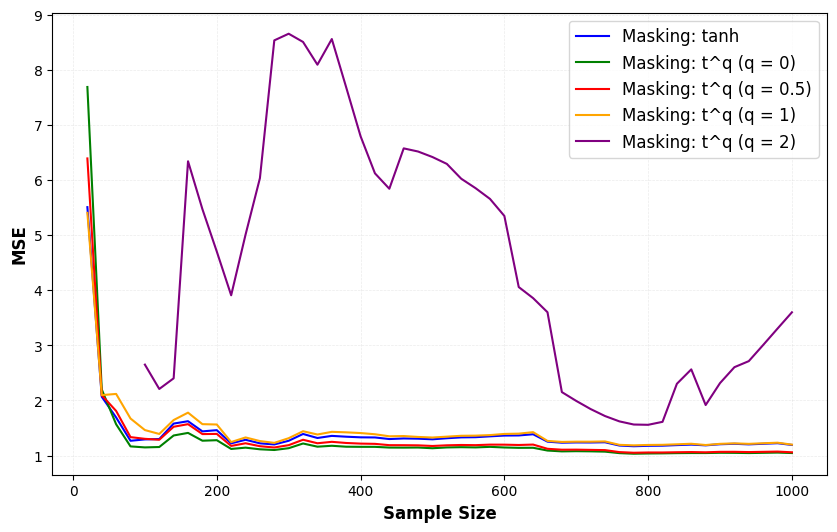
\includegraphics[width=0.8\textwidth]{images/Figure 17.png}
    \captionsetup{format=hang, singlelinecheck=false}
    \caption{Effect of sample size on mean shift regularization with weighted gradient descent (step size, $\gamma = 0.1$ and number of iterations $=7500$) using self-attention mechanism. Here, we use different masking functions, both unbounded and bounded.}
    \label{fig:17}
\end{figure}

In Figure \ref{fig:17}, we observe that with same sample size ($n = 1000$), unbounded masking function with low value of $q$ ($q=0.5$) gives the best result for low sample sizes. We note here that the green line corresponding to $q=0$ is the unweighted gradient descent here. For higher sample sizes ($>800$), the performance of most masking functions are almost similar with very less difference. We can easily observe that the only exception is the unbounded masking function $m_q(t) = t^q$ with highest value of $q$ ($q=2$), because high value of $q$ leads to unstable learning process. This aligns with our observation from Figure \ref{fig:16} and theoretical expectations discussed in section \ref{choice-masking-q} (Choice of Masking Function). 
\chapter{Conclusion}\label{chp:7}

Our experimental setup investigates the impact of covariate shift in linear regression models, particularly focusing on how a shift in the input mean affects Mean Squared Error (MSE) for different estimators. The study is conducted using both Ordinary Least Squares (OLS) and Gradient Descent (GD) estimators, followed by regularization techniques like importance weighting using Kernel Density Estimation (KDE) and a Self-Attention Mechanism.\\

The experiments confirm that covariate shift significantly impacts model performance, particularly for standard estimators like OLS. Gradient Descent adapts better to shift conditions, especially when combined with importance weighting techniques. Regularization methods, such as kernel-based importance weighting and self-attention mechanisms, effectively reduce MSE, making them valuable strategies for mitigating the negative effects of distributional shifts. It was also found that sample size and proper selection of masking function in self-attention mechanism also plays a crucial role in the rate of convergence in regularizing the effect of covariate shift.\\

These findings highlight the necessity of incorporating robust adaptation techniques in machine learning models deployed in real-world scenarios where covariate shift is prevalent.



% Bibliography Section
% \bibliographystyle{ieeetr}            % Style for bibliography
% \bibliographystyle{unsrt}             % Style for bibliography
% \bibliographystyle{alpha}             % Style for bibliography
\bibliographystyle{apalike}
\bibliography{bibliography}             % References in bibliography.bib

\end{document}
